\documentclass[a4paper,english,10pt]{report}


%\usepackage[french]{babel}
\usepackage[utf8]{inputenc}		% french special caracters (é, è, à, ...)
\usepackage[pdftex]{graphicx}				% to include figure in the document
\usepackage[footnotesize]{caption}      	% caption of table and figure in footnote size
\usepackage{color}                     			% texte en couleurs
\usepackage{subfig}					% allow the use of subfigure in the figure environment
\usepackage{fancyhdr}				% change header and footer
\usepackage{hyperref} 				% make hyperref in the pdf document
\usepackage{geometry}  				% change de geometry of the page
%\usepackage{eurosym}				% use of euro symbol
%\usepackage{floatflt}   				% for floating figure
\usepackage{multirow}
\usepackage[Glenn]{fncychap}            	% formatage des titres de chapitres
\usepackage{fancyvrb}                   		% pour afficher du code
%\usepackage{amsmath}				% math package
\usepackage{sidecap}				% caption at le left or right side of the figures
%\usepackage{lettrine} 				% emploi de lettrine au debut du chapitre
\usepackage{url}
\usepackage{makeidx}


\geometry{a4paper,tmargin=3cm,bmargin=2.5cm,lmargin=4cm,rmargin=3cm}
\pagestyle{headings}
\fancyfoot[C]{  \thepage \ }
\bibliographystyle{apalike}
\makeindex


%==========================pour les images================================
\graphicspath{{images/graphes/},{images/diagrammes/},
{images/illustrations/}, {images/}}
\DeclareGraphicsExtensions{.jpg,.png, .tiff, .pdf}

%==========================numérotations==================================
\setcounter{tocdepth}{1}                % affiche jusqu'aux susubsections dans toc
\setcounter{secnumdepth}{3}             % chapitres et sections numrots
\setlength{\tolerance}{1000}             % tolrance pour l'espace entre les mots

%==========================pour les couleurs===============================
\definecolor{coolRed}{RGB}{223,0,0}
\definecolor{coolBlue}{rgb}{0.2,0,0.5}
\definecolor{coolSection}{RGB}{50,109,50}
%\definecolor{coolSection}{RGB}{64, 127, 0}
\definecolor{red}{RGB}{255,0,0}
\definecolor{coolSubSection}{RGB}{0,0,0}
\definecolor{coolYellow}{RGB}{254,203,1}
\definecolor{coolGreen}{RGB}{22,109,15}

%=======================en-tête et pieds de page==================================

\pagestyle{fancy}
\fancyhf{}
\fancyhead[L]{\leftmark}
\fancyfoot[R]{\thepage}

%==================== DOCUMENT =================================


\begin{document}

%-----------------------------TITRE---------------------------------

\thispagestyle{empty}
~
\vspace {75mm}

\begin{flushright}

\begin{figure}[!h]
\hspace{10mm} 
\includegraphics[width=14cm]{SmartRoot_logo}
\end{figure}

{\Large version 4.1}
\hspace{5mm}\\
\vspace{10mm}
{\color{coolSection}\rule{145mm}{3mm}}\\
%{\color{coolYellow}\rule{145mm}{3mm}}\\ 

\end{flushright}


\vspace{5mm}


\begin{flushright}
\vspace{5mm}
{\large Software created by Xavier Draye and Guillaume Lobet}\\ 
xavier.draye@uclouvain.be\\
\vspace{5mm}
{\large Manual written and maintained by Guillaume Lobet}\\ 
guillaume.lobet@ulg.ac.be\\
\end{flushright}

\vspace{10mm}

\begin{center}
\vfill
{\large \today} 
\end{center}

~~
\newpage
~~
\vspace{13cm}

SmartRoot is a semi-automated image analysis software which streamlines the quantification of root growth and architecture for complex root systems. The software combines a vectorial representation of root objects with a powerful tracing algorithm which accommodates to a wide range of image source and quality. In its vectorial form, the root system is treated as a collection of roots (possibly connected) that are individually represented as parsimonious sets of connected segments. Pixel coordinates and grey level are therefore turned into meaningful biological attributes such as segment diameter and orientation, distance to any other segment or topological location. As a consequence, user interaction and data analysis directly operate on root segments and are not hampered by the spatially discrete, pixel-based nature of the original image. The software supports a sampling-based analysis of root system images, in which detailed information is collected on a limited number of roots selected by the user according to specific research requirements. SmartRoot is an operating system independent freeware based on ImageJ and uses cross-platform standards for communication with data analysis softwares.\\

More precise explanation about SmartRoot algorithm can be found in the following paper:\\

\noindent \fbox{\parbox{\linewidth}{ \href{http://www.plantphysiol.org/content/157/1/29.abstract?sid=6c3bae80-1a8d-4fc6-9d70-34e2f8e4ba03}{\textbf{A Novel Image Analysis Toolbox Enabling Quantitative Analysis of Root System Architecture.}\\
Guillaume Lobet, Loic Pagès and Xavier Draye. \\
2011, Plant Physiology, 157, pp 29-39}}}

~~
\newpage
~~
%\vfill
%\vspace{13cm}
%\begin{figure}[htbp]
%\begin{center}
%
\includegraphics[width=\linewidth]{logo_ucl_eli.pdf}
%\end{center}
%\end{figure}	
%
%\newpage

%-----------------------------RESUME---------------------------------

\tableofcontents
\listoffigures


~~
\newpage


\chapter{SmartRoot Installation}
\label{install}



{\color{coolSection}\section{First steps}}

{\color{coolSubSection}\subsection{System requirement}}

\begin{description}
\item [Memory:] At least 1024 MB of RAM for a good functioning
\item [Java:] SmartRoot works with Java 1.5 or higher
\item [Database (optional):] SmartRoot can export data to .csv text files but also directly into a database. For Windows we present how to setup a MS Access database connection. For Mac OS X and Linux (Ubuntu), we present how to setup a MySQL connection. People who does not have MS Access on Windows can follows similar steps as for Linux and Mac OS to install a MySQL database.
\end{description}

%%%%%%%%%%%%%%%%%%%%%%

{\color{coolSubSection}\subsection{Installation files}}

\noindent Inside the SmartRootSetup.zip file, you will find the following folders and files:\\

\begin{description}
\item [SmartRoot Quick Start.pdf] This document. Helps you to quickly install SmartRoot.
\item[SmartRoot User Guide.pdf] Complete user guide to learn all the SmartRoot functionalities. 
\item [Quick Start Images folder] Four images to learn how to trace root with SmartRoot. Instructions are written directly on the images.
\item [SmartRoot folder] The SmartRoot program in itself. Contains four .jar files: Smart\_Root.jar, Image\_Explorer.jar, jcommon-1.0.16.jar, jfreechart-1.0.13.jar and mysql-connector-java-5.1.7-bin.jar. This is the folder you will have to copy in the ImageJ folder (see below).
\end{description}

%%%%%%%%%%%%%%%%%%%%%%

\newpage
{\color{coolSection}\section{Windows installation}}

\begin{enumerate}
\item Configure the database (optional)
\item Install ImageJ and SmartRoot
\item Use the Quick start images
\end{enumerate}

%{\color{coolSubSection}\subsection{Java 1.5 installation}}
%
%Download Java 1.5 from the following page (choose the Java Runtime Environment (JRE) 5.0 Update 22) and install it.\\
%
%\noindent \fbox{\parbox{\linewidth}{\url{http://java.sun.com/javase/downloads/index_jdk5.jsp}}}\\ 

{\color{coolSubSection}\subsection{Database installation and connection}}
\label{dbwin}

\noindent To configure an ODBC data source that connects SmartRoot to a MS Access database:\\

\begin{enumerate}
\item Close the ImageJ program if it is running
\item Starts the \verb|ODBC administrator| from the \\ \verb|Control panel > Administrative tools > ODBC administrator|
\item Under the tab \verb|User DSN|, click \verb|Add…|
\item A list of database drivers is displayed. Select \verb|Microsoft Access Driver|, and click \verb|Finish|. You may need to contact your DB vendor if the driver is not in that list.
\item In the next dialog box, specify \verb|SmartRoot| in the \textbf{Data Source Name} field. In the \textbf{Database} area, click \verb|Create| to create a new database. Choose the directory in which you want to create the database, and name it \verb|SmartRoot.mdb| (in the upper left text field).
\item Click OK to validate and quit the ODBC administrator.\\
\end{enumerate}

When you launch SmartRoot (see below), the following message is displayed in the Results window of ImageJ if the connexion was successfully established:

\begin{Verbatim}[frame=single, commandchars=+\(\)]
SQL connection started on ODBC source SmartRoot
\end{Verbatim}

If the program failed to open the datasource, the message is:

\begin{Verbatim}[frame=single, commandchars=+\(\)]
The ODBC datasource 'SmartRoot' was not found.
You will not be able to write to a database.
\end{Verbatim}

{\color{coolSubSection}\subsection{SmartRoot installation\\}}

\begin{enumerate}
\item Download and install ImageJ 
\item Copy the SmartRoot folder in the \verb|Program Files > ImageJ > Plugins| folder.
\item Open ImageJ and choose \verb|Plugins > SmartRoot > SR Explorer|\\
\end{enumerate}

\noindent ImageJ download:\\

\noindent\fbox{\parbox{\linewidth}{\url{http://rsbweb.nih.gov/ij/download.html}\\
\footnotesize{If you do not have Java installed, please choose a version of ImageJ bundled with Java}}}\\\\

\noindent
\fbox{\parbox{\linewidth}{%
{\color{red}\textsc{Important:}}\\
If you are using {\color{coolSection} Windows 7}, all the components you are using together (in our case, Java, ImageJ and Access) have to be build on the same architecture (32bit or 64bit). \\
\noindent For instance,  if your Access software is 64bit, please choose the {\color{coolSubSection}ImageJ bundled with 64 bit Java} in the ImageJ download page. 
}}\\

%%%%%%%%%%%%%%%%%%%%%%%%%%%%%

\newpage

{\color{coolSection}\section{Mac OSX installation}}

\begin{enumerate}
\item Install and configure MySQL database (optional)
\item Install ImageJ and SmartRoot
\item Use the Quick start images
\end{enumerate}

{\color{coolSubSection}\subsection{MySQL installation and configuration}}
\label{dbmac}

\subsubsection{Installation}
Download the latest MySQL version from:\\ 

\noindent \fbox{\parbox{\linewidth}{\url{http://dev.mysql.com/downloads/}}}\\

\noindent
Open the disk image then install MySQL by double clicking on the \verb|mysql-...-.pkg| icon. \\
Also install the \verb|MySQLStratupItem.pkg| and \verb|MySQL.prefPane|.\\

\noindent
Open the \verb|System Preferences>MySQL| and start the MySQL server.

\subsubsection{Configuration}

Download the MySQLWorkbench from the following link and install it \\

\noindent \fbox{\parbox{\linewidth}{\url{http://dev.mysql.com/downloads/workbench}}}\\

\noindent 
Open the application and click \verb|New Connection|. Fill the fields as follow:\\

\noindent
\fbox{ \parbox{\linewidth}{%
\textbf{Connection Name:} choose the name you want (ex: SmartRoot) \\ 
\textbf{Connection Method:} Standart (TCP/IP)\\
\textbf{Hostname:} localhost \\ 
\textbf{Port:} 3306 \\ 
\textbf{Username:} choose the name you want (ex: root) \\ 
\textbf{Password:} leave it empty \\ 
\textbf{Default Schema:} leave it empty }} \\

\noindent
Open the connection and create a new schema called \verb|SmartRoot| by clicking the '+' sign.\\
Name the new schema SmartRoot and create it. \\
Click the \verb|Refresh| button to see your newly created database.


{\color{coolSubSection}\subsection{SmartRoot installation \\}}

\begin{enumerate}
\item Download and install ImageJ 
\item Copy the SmartRoot folder in the \verb|Applications > ImageJ > Plugins| folder.
\item Open ImageJ and choose \verb|Plugins > SmartRoot > SR Explorer|\\
\end{enumerate}

\noindent ImageJ download:\\

\noindent\fbox{\parbox{\linewidth}{\url{http://rsbweb.nih.gov/ij/download.html}}}

\newpage
{\color{coolSubSection}\subsection{Connect SmartRoot to the database}}

Once you have installed SmartRoot, open it.
The following message is displayed in the Results window of ImageJ if the connexion was successfully established:\\

\begin{Verbatim}[frame=single, commandchars=+\(\)]
SQL connection started 
\end{Verbatim}

\noindent If the program failed to open the datasource, the message is:

\begin{Verbatim}[frame=single, commandchars=+\(\)]
The specified datasource was not found.
You will not be able to write to a database.
\end{Verbatim}

\noindent
If you see this error message, go in the SmartRoot window, choose the \verb|Settings| tab and find the \verb|SQL options| panel. Fill the fields as follow:\\

\noindent
\fbox{\parbox{\linewidth}{%
\textbf{Driver class name:} com.mysql.jdbc.Driver\\
\textbf{Connection URL:} jdbc:mysql://localhost/SmartRoot\\
\textbf{Connection user name:} the username you choose previously\\
\textbf{Connection password:} leave empty }}\\
	
\noindent Press the \verb|Save Prefs| then \verb|Restart server| button. You should see the correct message saying the connection started


%%%%%%%%%%%%%%%%%%%%%%%%%%%%%%%%%%%%
\newpage
{\color{coolSection}\section[Linux installation]{Linux installation (Ubuntu distribution)}}

\begin{enumerate}
\item Install MySQL (optional)
\item Install ImageJ
\item Install ImageJ and SmartRoot
\item Configuring the database (optional)
\item Use the Quick start images
\end{enumerate}

%{\color{coolSubSection}\subsection{Java 1.5 installation}}
%
%In the terminal window type:\\
%
%\begin{Verbatim}[frame=single, commandchars=+\(\)]
%$sudo apt-get install sun-java5-jre
%\end{Verbatim}


{\color{coolSubSection}\subsection{MySQL installation and configuration}}
\label{dblin}

\subsubsection{Installation}

In the terminal window type:\\

\begin{Verbatim}[frame=single, commandchars=+\(\)]
$sudo apt-get install mysql-server
$sudo apt-get install mysql-query-browser
\end{Verbatim}

\noindent
While installing, you will be asked to setup username and password for your database connection. Leave the default values.

\subsubsection{Configuration}

Open MySQL Administrator. To connect to the database fill the form as follow:\\

\noindent
\fbox{\parbox{\linewidth}{%
\textbf{Server Hostname:} localhost\\
\textbf{Username:} root\\
\textbf{Password:} Leave empty}}\\

\noindent
In the MySQL Administrator window, choose \verb|Catalog| in the left panel. 

\noindent
In the bottom left panel \verb|Schemata|, right-click and choose \verb|Create Schema|. \\
Name it \verb|SmartRoot|



{\color{coolSubSection}\subsection{ImageJ installation}}

\noindent
In the terminal window type:\\

\begin{Verbatim}[frame=single, commandchars=+\(\)]
$sudo apt-get install imagej
\end{Verbatim}



{\color{coolSubSection}\subsection{SmartRoot installation}}

Copy the \verb|SmartRoot| folder from the \verb|SmartRootSetup| folder you downloaded into the \verb|usr/share/imagej/plugins/| folder\\

\noindent
In the terminal window type:\\

\begin{footnotesize}
\begin{Verbatim}[frame=single, commandchars=+\(\)]
$sudo mv /home/(+color(red)where_you_unzipped)/SmartRootPlug/SmartRoot /usr/share/imagej/plugins
\end{Verbatim}
\end{footnotesize}

\noindent To launch SmartRoot open ImageJ and choose \verb|Plugins > SmartRoot > SR Explorer|\\

\noindent
\fbox{\parbox{\linewidth}{%
{\color{red}\textsc{Important:}}\\
Ubuntu use the {\color{coolSubSection}Alt-key} to grab and move windows. SmartRoot use the same key to automatically trace roots. In order to use SmartRoot correctly, you have to change one Ubuntu parameter:\\

\noindent Go to System $>$ Preferences $>$ Windows and set the Movement key to Super.}}\\


{\color{coolSubSection}\subsection{Connect SmartRoot to the database}}

Once SmartRoot is installed, open it.

\noindent
The following message is displayed in the Results window of ImageJ if the connexion was successfully established:\\

\begin{Verbatim}[frame=single, commandchars=+\(\)]
SQL connection started 
\end{Verbatim}

\noindent If the program failed to open the datasource, the message is:

\begin{Verbatim}[frame=single, commandchars=+\(\)]
The specified datasource was not found.
You will not be able to write to a database.
\end{Verbatim}

\noindent
If you see this error message, go in the SmartRoot window, choose the \verb|Settings| tab and find the \verb|SQL options| panel. Fill the fields as follow:\\

\noindent
\fbox{\parbox{\linewidth}{%
\textbf{Driver class name:} com.mysql.jdbc.Driver\\
\textbf{Connection URL:} jdbc:mysql://localhost/SmartRoot\\
\textbf{Connection user name:} the username you choose previously (default = root)\\
\textbf{Connection password:} leave empty }}\\
	
\noindent
Press the \verb|Save Prefs| then \verb|Restart server| button. You should see the correct message saying the connection started

%%%%%%%%%%%%%%%%%%%%%%%%%%%%%%%%%%%%%%%%%







%----------------------
%%%%%%%%%%%%%%%%%%%%%%%%%%%%%
%%%%%%%%%%%%%%%%%%%%%%%%%%%%%

\chapter{Introducing SmartRoot}

%%%%%%%%%%%%%%%%%%%%%%%%%%%%%

{\color{coolSection}\section{SmartRoot versus other root image analysis software}}

SmartRoot differs from most root image analysis software in that it does not use traditional raster-based morphological operations (such as skeletonizing) to extract roots structures. SmartRoot uses vector-based and interactive algorithms to detect root objects. Each root object consists of a polyline (an open polygon) with a name, and whose thickness (root diameter) is estimated at each node. The polyline coordinates, diameters and other features are stored in a DataFile in the XML format. Because it is vector based, SmartRoot has a potential for higher resolution than raster-based. Because it is interactive, the human eye and hands are involved in the tracing of roots, which makes the algorithm powerful yet time consuming at the same time. Therefore, and although this problem could be worked around in future versions, SmartRoot may not be suited to exhaustive analyses of whole root systems comprised of hundreds of roots.\\

Another difference between SmartRoot and other systems is that the objects are displayed in different layers than the root image itself. The root image is therefore not modified during tracing of roots, and it is possible to show/hide the various features of the objects: root axis, root border, root area, root nodes (nodes of the polyline showing the root diameter) or a ruler along roots. This also allows to remove or modify any root object.\\

%%%%%%%%%%%%%%%%%%%%%%%%%%%%%

\newpage
{\color{coolSection}\section{The windows of the ImageJ / SmartRoot user interface}}
\label{sr-ij}

\begin{description}
\item [The ImageJ window] The native window of ImageJ. It allows the user to select SmartRoot tools and to perform image manipulations on images during a SmartRoot session (see \ref{ijfunc}).

\item [SmartRoot Explorer] An "image browser" which displays the list of image files in the file system. Image windows are opened by double-clicking an image item in the list. Several images can be opened concurrently. Images have to be open with this window to be recognize by SmartRoot

\item [Image windows] Display the working images. To access functions of SmartRoot, one uses the mouse right button within the area of an Image window, which brings up a contextual popup menu.

\item [Results window] Displays some notes / error messages on the execution of SmartRoot.

\item [SmartRoot window] Comprises seven tabs (see chap. \ref{tabs} for detailed description). 
	\begin{description}
	\item [Layout tab] Select the attributes to be displayed. 
	\item [Root List tab]Visualize all the traced roots and marks of the image. 
	\item [Linked files tab] Import data from other image (see \ref{chaplink}).
	\item [Data Transfer tab] Send the data to an external database or to a .csv file (see \ref{chaptrans}).
	\item [Plot tab] Plot several data of the current image (see \ref{chapplot})
	\item [Settings tab] Change the settings such as the resolution or the root names
	\item [About tab] Learn about SmartRoot
	\end{description}
\end{description}

\begin{figure}[!hbtp]
\begin{center}
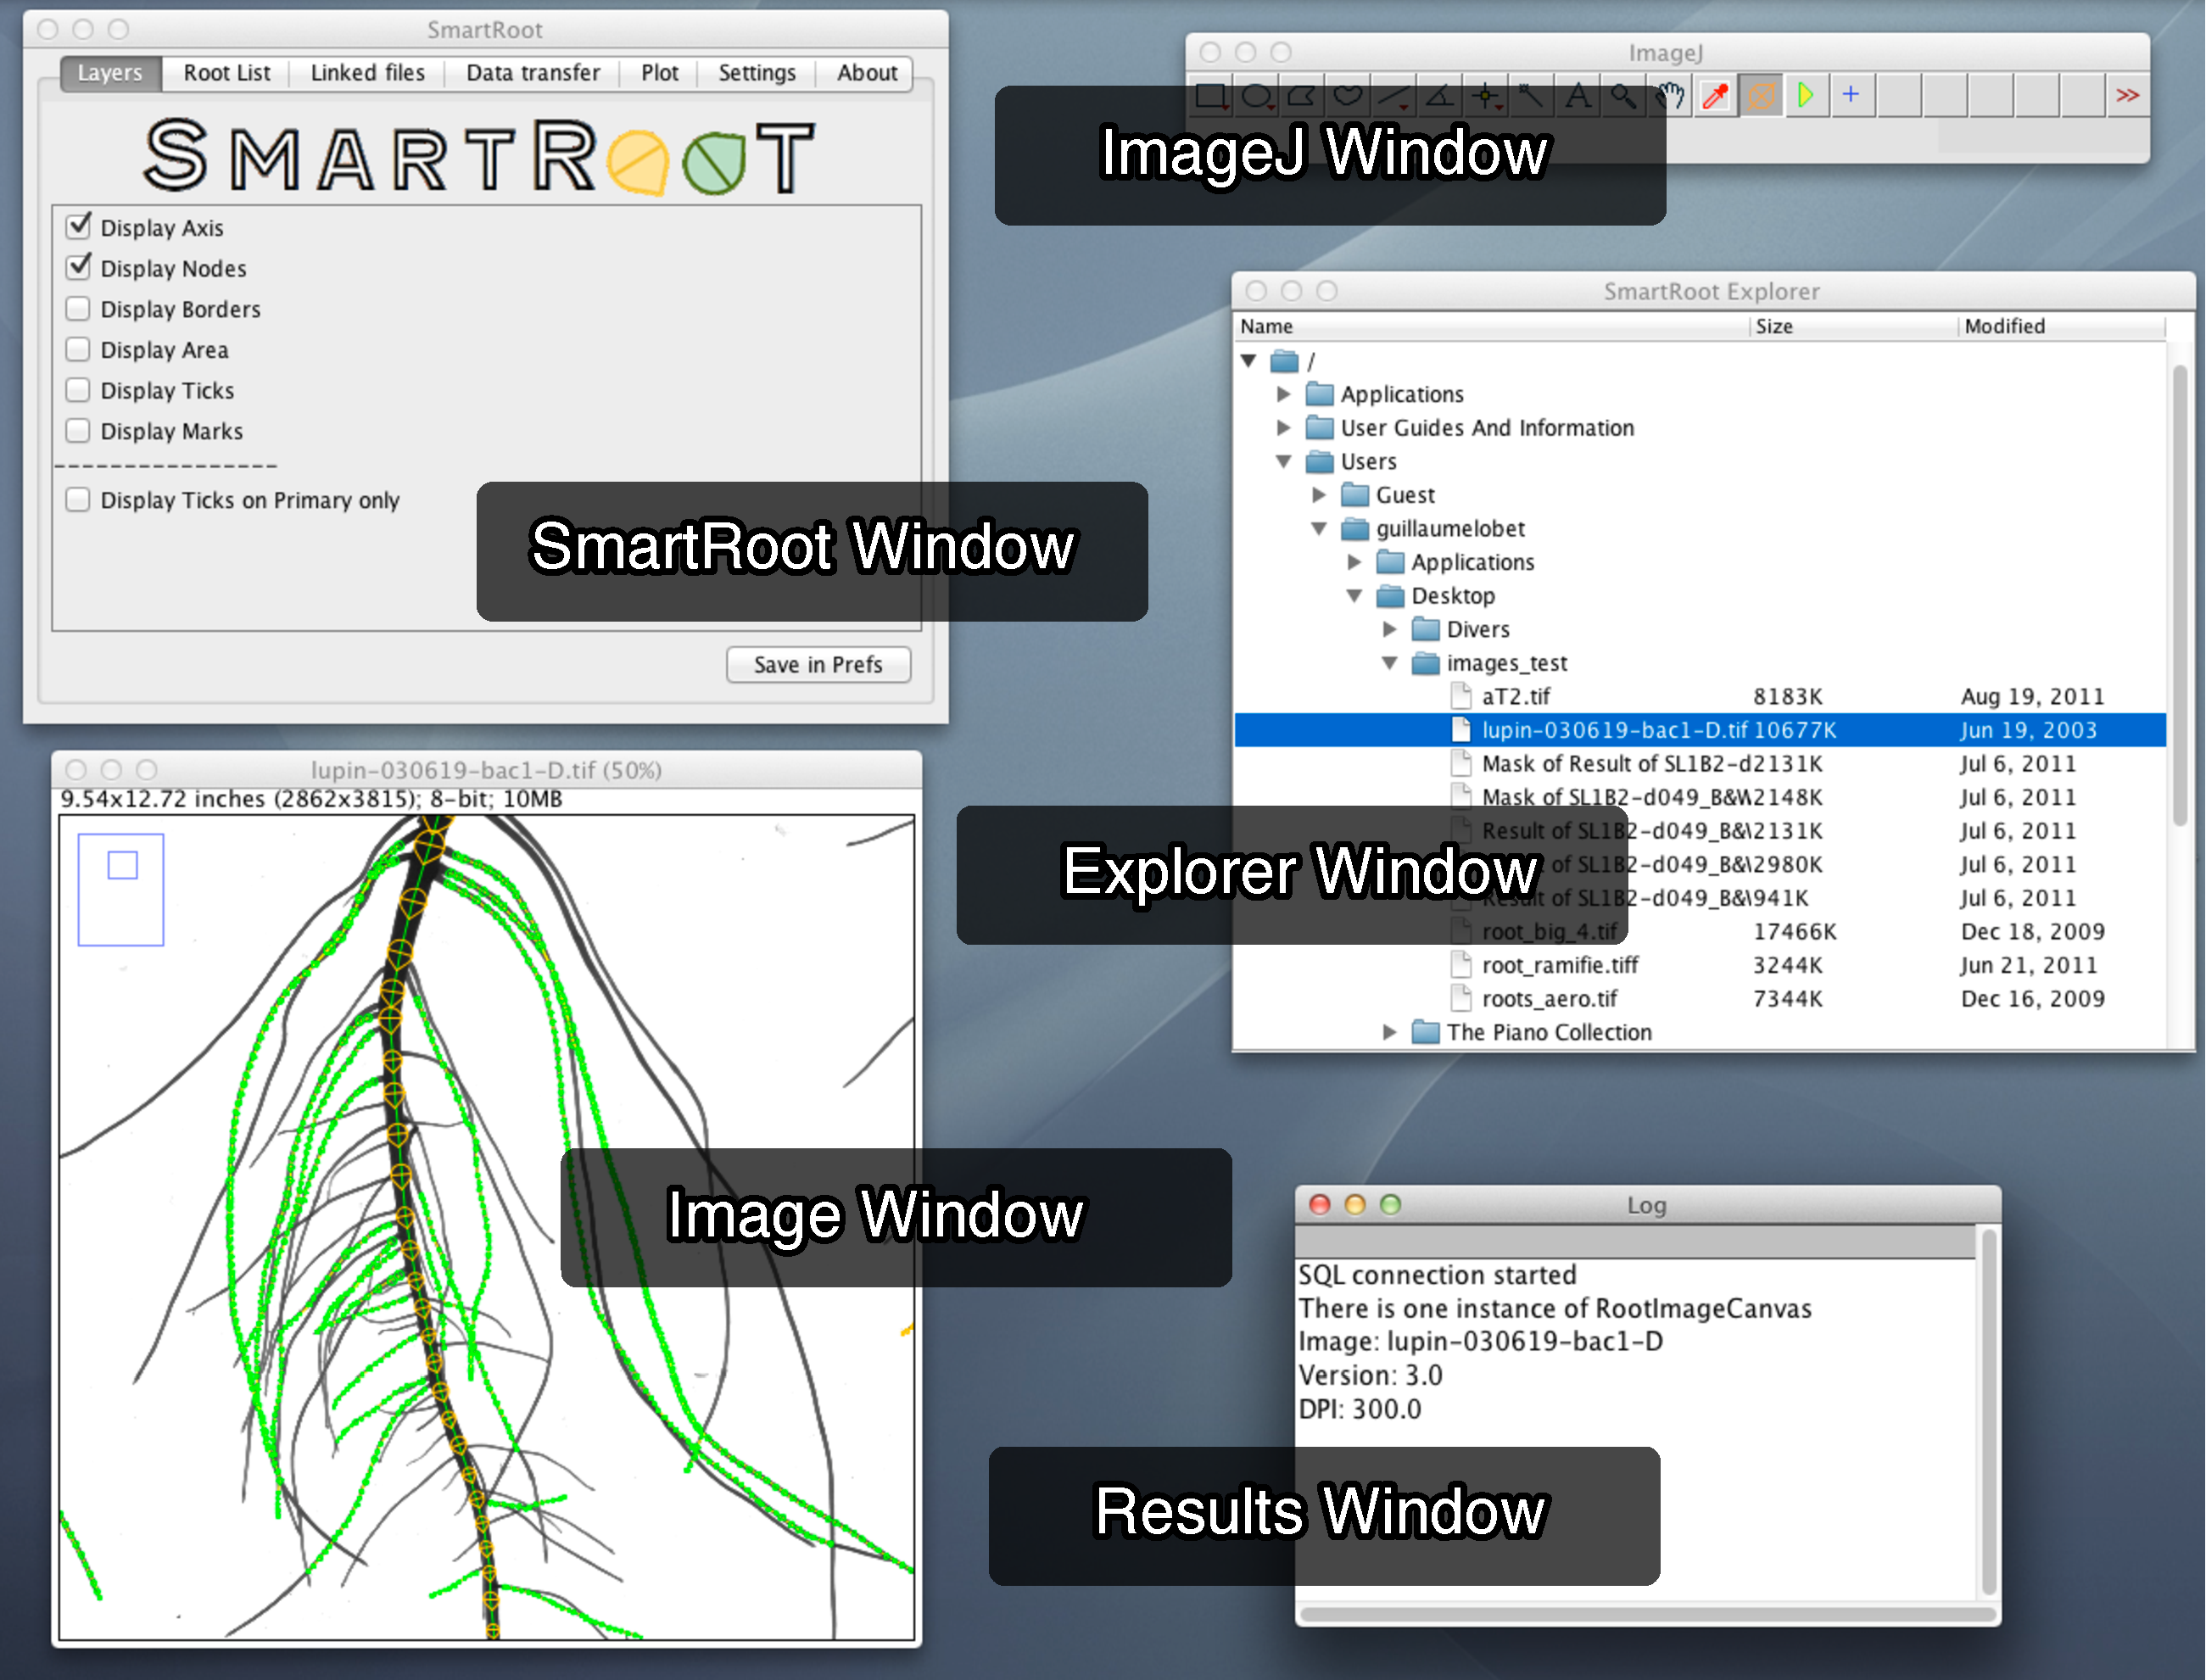
\includegraphics[width=0.9\linewidth]{SR_windows_1}
\caption[]{\textbf{SmartRoot different windows}}
\label{sr_win}
\end{center}
\end{figure}
%%%%%%%%%%%%%%%%%%%%%%%%%%%%%
%%%%%%%%%%%%%%%%%%%%%%%%%%%%%

\chapter{Using SmartRoot}

{\color{coolSection}\section{Quick start tutorial}}

Together with SmartRoot comes a Quick start tutorial made of four images. All instructions to analyze these images are written on the images themselves and, at the end of this short tutorial, you will be able to use all the main functions of SmartRoot.

%%%%%%%%%%%%%%%%%%%%%%%%%%%%%

{\color{coolSection}\section{Opening images}}

To work on a root image, you have to open it with the Explorer Window of SmartRoot (see figure \ref{sr_win}, the window on the right side).\\

\noindent
\fbox{\parbox{\linewidth}{%
{\color{red}\textsc{Important:}}\\
 If you open an image with the ImageJ regular file opener (File$>$Open or drag and drop), the image will not be recognize by SmartRoot and you will not be able to trace roots.}}\\


{\color{coolSection}\section{Preparing images}}

SmartRoot only processes grayscale (8-bit) images. If you attempt to open an image that is not of grayscale type, a warning message will be displayed that the image will be converted to grayscale and you will be invited to save the new (converted) image (which is not mandatory if you prefer to reconvert the image every time you work on it).\\

The current implementation assumes roots have lower pixel (darker) values than the background (the Status line in the ImageJ window indicates the value of the pixel under the mouse cursor). If the value of root pixels appears to be higher than that of background pixels, you should use the \verb|Edit > Invert| command of ImageJ before proceeding to root tracing.\\

Keep in mind that the screen grey level may be inverted relative to the pixel values, depending on the current Lookup table (i.e. a table which assigns screen grey levels to pixel values). The \verb|Image > Lookup Table > Invert| LUT command of ImageJ allows you to reverse the screen greyscale without changing the pixel values.

%%%%%%%%%%%%%%%%%%%%%%%%%%%%%%%%%%%

\chapter{SmartRoot tools}

{\color{coolSection}\section{Overview of SmartRoot Tools}}

SmartRoot uses six different tools: the trace, the mark, the line, the zoom, the hand and the registration anchor. To switch from one tool to another, use either the contextual (right-button) popup menu inside the image or the corresponding icons in the ImageJ window.
\index{tools}

\begin{figure}[h]
\centering
   \subfloat[]{\label{line}
\includegraphics[width=1cm]{line}}
  \hspace{5mm}   
   \subfloat[]{\label{zoom}
\includegraphics[width=1cm]{zoom}}
  \hspace{5mm}   
  \subfloat[]{\label{hand}
\includegraphics[width=1cm]{hand-1}}
  \hspace{5mm}   
  \subfloat[]{\label{trace}
\includegraphics[width=1cm]{trace}}
  \hspace{5mm}  
    \subfloat[]{\label{lattrace}
\includegraphics[width=1cm]{lattrace}}
  \hspace{5mm}      
  \subfloat[]{\label{regancor}
\includegraphics[width=1cm]{regancor}}
  \hspace{5mm}   
    \subfloat[]{\label{mark}
\includegraphics[width=1cm]{mark}}
  \hspace{5mm}  
  
\caption[SmartRoot tools]{\textbf{SmartRoot tools}. (a) Line tool (b) Zoom tool (c) Hand tool (d) Trace tool (e) Lateral trace tool (f) Registration Ancor tool (g) Mark tool }
\label{apoplastique}
\end{figure}

\begin{description}

\item [Line tool] If the user draw a line crossing several roots, he can use the function \verb|Automatic drawing| in the right-click menu. This function will start tracing all the roots crossing the line. 

 \item [Zoom tool] The left and right mouse buttons zoom in and out, respectively. To switch from the zoom tool to another tool, either use the ImageJ icons or press the escape key (which brings you back to the crosshair tool).

\item[Hand tool] Moves the image in the window. When the crosshair or the zoom tool is active, you can transiently switch to the hand tool by holding the space bar down (as in Photoshop). This allows you for example to access the non visible part of a large image while tracing a root.

\item[Trace tool] Used for all root objects manipulations (drawing, selecting; moving…) (see sec. \ref{traceTool})

\item[Lateral Trace tool] Used to trace lateral roots along a traced first order root.

\item[Registration Anchor tool] Used to add anchor points that will be used to align time-series of images.

\item[Mark tool] Used to add marks along roots. These marks can be exported all at once to the database from the Data transfer tab of the SmartRoot window.
\end{description}

%----------------------------
%----------------------------

{\color{coolSection}\section{The Trace tool}}
\label{traceTool}

\subsection{Manual tracing procedure}
\label{manualTrace}

Root tracing is best illustrated with the basic, most inefficient way (yet sometimes necessary) of tracing a root, viz. tracing a polyline manually along the axis of the root, as you would do with any drawing software. \\

Before tracing your first root, select the Trace tool (either from the popup menu within your image, or from the toolbar of ImageJ) and make sure the \verb|Display nodes| and \verb|Display axis| items of the \verb|Layers| tab in the SmartRoot window are checked so you can see what you are drawing. \\

To start tracing, place the cursor close to the base of the root (within the root) and click the left button to insert a "node" there. Then proceed drawing the polygon with successive clicks. Each node is displayed as a "drop" symbol whose diameter approximates the root diameter at the node location and whose orientation indicates the direction of drawing. You will notice that SmartRoot always tries to keep the node that you are tracing in the center of the root, even if the mouse if not in the center (see \ref{escape} to control this behavior). \\ 

To insert the last node of the polygon, make a double-click. By default, SmartRoot assumes you have traced the root from the base to the apex. The root apex is represented with a filled yellow circle. You are then invited to enter a name for that root (the reason for this will be obvious later). If you press Cancel, the tracing will be discarded.

\begin{figure}[htbp]
\begin{center}
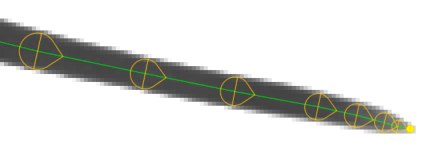
\includegraphics[width=10cm]{root-1}
\caption[Traced root]{\textbf{Traced root}}
\label{root-1}
\end{center}
\end{figure}


%------------------------------------
\subsection{Semi-automated tracing procedure}
\label{autoTrace}

SmartRoot offers more efficient ways to trace roots, in which algorithms attempts to trace the root polygon by itself. The algorithms are semi-automated in that they still requires some user input for each root. Semi-automatic tracing starts whenever the user press the {\color{coolBlue}\verb|Alt|} key when inserting a node.

If you press the {\color{coolBlue}\verb|Alt|} key when creating the first node of a root, SmartRoot will trace a new root in both directions from that node. Because the algorithm needs to guess the root direction, it is recommended not to trace the first node just at the intersection between two roots.

If you press the {\color{coolBlue}\verb|Alt|} key when you insert the $n^{th}$ node (n $>$ 1) of a root (manual tracing), SmartRoot switches to semi-automatic tracing and proceeds until it reaches the end of the root.

%------------------------------------
\newpage
\subsection{Modifying a root}
\label{modify}

Once a root has been traced, it can be modified in a number of ways.\\

To \textbf{move a single node}, just click within the area of the node symbol and drag it with the mouse to the desired location. If you hold the {\color{coolBlue}\verb|Alt|} key (semi-automatic) while releasing the mouse button, the distal part of the root will be completely reconstructed (unless you are moving the first node of a root, in which case SmartRoot elongates the root proximal to that node).\\
 
The \textbf{other modifications} of root objects are requested by clicking with the right button on the root node to be modified (within the node symbol area) or anywhere in the root to be modified (within the area enclosed by the root borders), then choosing the desired action in the popup menu that shows up. This will bring up a popup menu whose first items (unselectable, yellow background) indicates the name of the selected root, the name of its parent (if applicable) and the ramification order of the root.\\


\noindent \underline{\textbf{If you select a node:}}\\

\begin{description}
\item[Append nodes:] this item will be selectable only if the selected node is either the first or the last node of a root object. After selecting this item, the user is left as if he was tracing the root in the manual tracing mode (with the possibility to connect the root to the base / end of an existing root and that to switch to the semi-automated tracing mode).
\item[Split root:] splitting a root actually creates two roots: the proximal part is stored in the original root object, while the distal part is stored in a new root object with the default name "unnamed".
\item[Remove node:] this will remove the selected node, linking (in any) the previous node to the next node.
\item[Remove all nodes (after):] this item will discard all node located distal to the selected node.
\item[Remove all nodes (before):] this item will discard all node located proximal to the selected node.\\
\end{description}

\noindent \underline{\textbf{If you select a root:}}\\

\begin{description}

\item[Bring to front:] this item will bring the selected root to the front of the list of roots. By default, every time a root is created, it is added at the front of the root list. Where roots overlap, only the root in front of the others can be selected. This command (and the next one) allows the user to move the selected root at the back or front of the root list.

\item[Send to back:] this item will send the selected root to the back of the list of roots.

\item[Find laterals:] this item will check along the root axis if there is lateral roots. Newly created laterals will be set as children of the selected root

\item[Fast find laterals:] Same function as \textbf{Find Laterals}, but using a other algorithm that is faster, but a little less efficient.

\item[Attach parent root:] this item set a parent for the current root (see sec.\ref{parentchild}). SmartRoot will display a list of all the available roots. The root closest from the base of the selected root will be set as first choice. The root selected in the list will be highlighted in red on the image (fig \ref{attachP}).

\begin{figure}[h]
\begin{center}
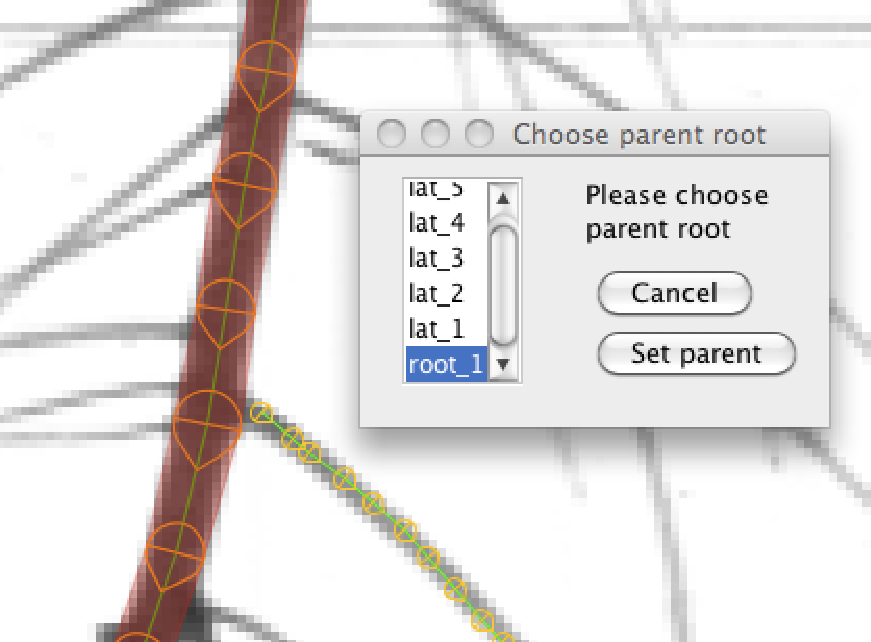
\includegraphics[width=5cm]{attachP}
\caption[Attaching parent]{\textbf{Attaching parent}. The root we want to attach a parent to is the one displayed in yellow. The red root is the one selected in the root list in the \textbf{Attach parent} dialog.}
\label{attachP}
\end{center}
\end{figure}

\item[Detach parent root:] this item remove the relationship between a root and its parent.

\item[Detach children roots:] this item remove the relationship between a root and all its children.

\item[Rename root:] this item will bring a dialog box to change the name of the selected root.

\item[Delete a root:] this item will remove the whole root. If the root has child(ren), the user will be asked if he wants to delete all the children or not. If not, the children will be detached.

\item[Reverse orientation:] this item will reverse the root orientation, changing the root base into the root apex and vice-versa.

\item[Crop childrens:] this item will cut all roots whose first node is located within the area of the selected root at their intersection with the border of the selected root, as shown on figure \ref{crop}.

\end{description}

\begin{figure}[h]
\centering
   \subfloat[]{\label{crop-1}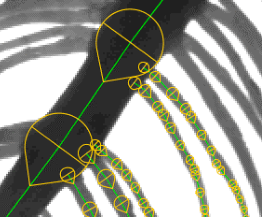
\includegraphics[width=4cm]{crop-1}}
  \hspace{5mm}   
  \subfloat[]{\label{crop-2}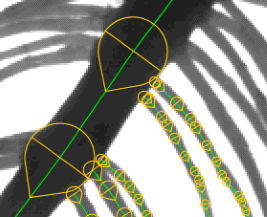
\includegraphics[width=4cm]{crop-2}}
  \hspace{5mm}   
  \subfloat[]{\label{crop-3}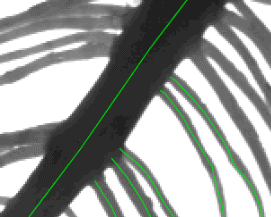
\includegraphics[width=4cm]{crop-3}}
\caption[Crop children]{\textbf{Crop children}. (a) Before cropping children (b) After cropping children (with nodes) (c) After cropping children (without nodes)}
\label{crop}
\end{figure}

%------------------------------------
\newpage
\subsection{Connecting two tracing}
\label{connecting}

There may be cases where you need to join two root objects that should make a single root. \\

If you want to join two drawings A \& B, make sure you the Trace tool is active, right-click the end of A, select \verb|Append node| and start adding nodes until you come close to the "start" of B, then add the last node of A using the right-click precisely on top of the first node of B, and you are done.  Note there is no requirement as to the orientations of A and B (you can append A by its base or apex, to the base or apex of B). The orientation of the resulting root will be that of A (you can reverse it as indicated in \ref{modify}). If the final orientation is A?B, the name of the resulting root will be that of A (and reverse).\\

On figure \ref{connect}, the top root is being traced (\ref{connect-1}) and an ultimate node is added onto the first node of the bottom root, automatically joining the two roots (\ref{connect-2}).

\begin{figure}[h]
\centering
   \subfloat[]{\label{connect-1}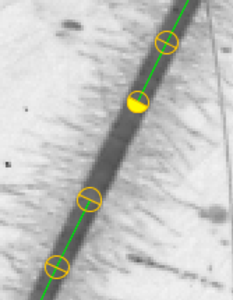
\includegraphics[width=2.5cm]{connect-1}}
  \hspace{10mm}   
  \subfloat[]{\label{connect-2}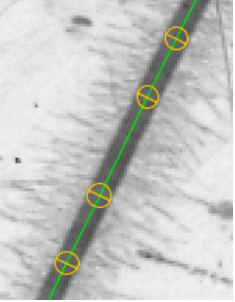
\includegraphics[width=2.5cm]{connect-2}}
\caption[Connecting roots]{\textbf{Connecting roots}. (a) Before connecting roots (b) After connecting roots}
\label{connect}
\end{figure}

%------------------------------------

\subsection{Topological informations}
\label{parentchild}

%\subsubsection{The parent / child relationship}


SmartRoot allow the user to set \textit{parent} and \textit{children} roots. Setting a root B as a parent of a second root B means B was created by A and is connected to it. \\

To connect two root with a topological link, select the child root and right-click on it. Choose \verb|Attach parent| and select the parent root in the list. The selected root in the list is highlight in red for better visualization. Once attached, roots of different ramification orders are displayed in different colors. When the user delete a root which has children, he will be asked if he wants to also delete the children. Stored topological informations are insertion position, insertion angles and ramification density.\\


%\begin{figure}[htbp]
%\begin{center}
%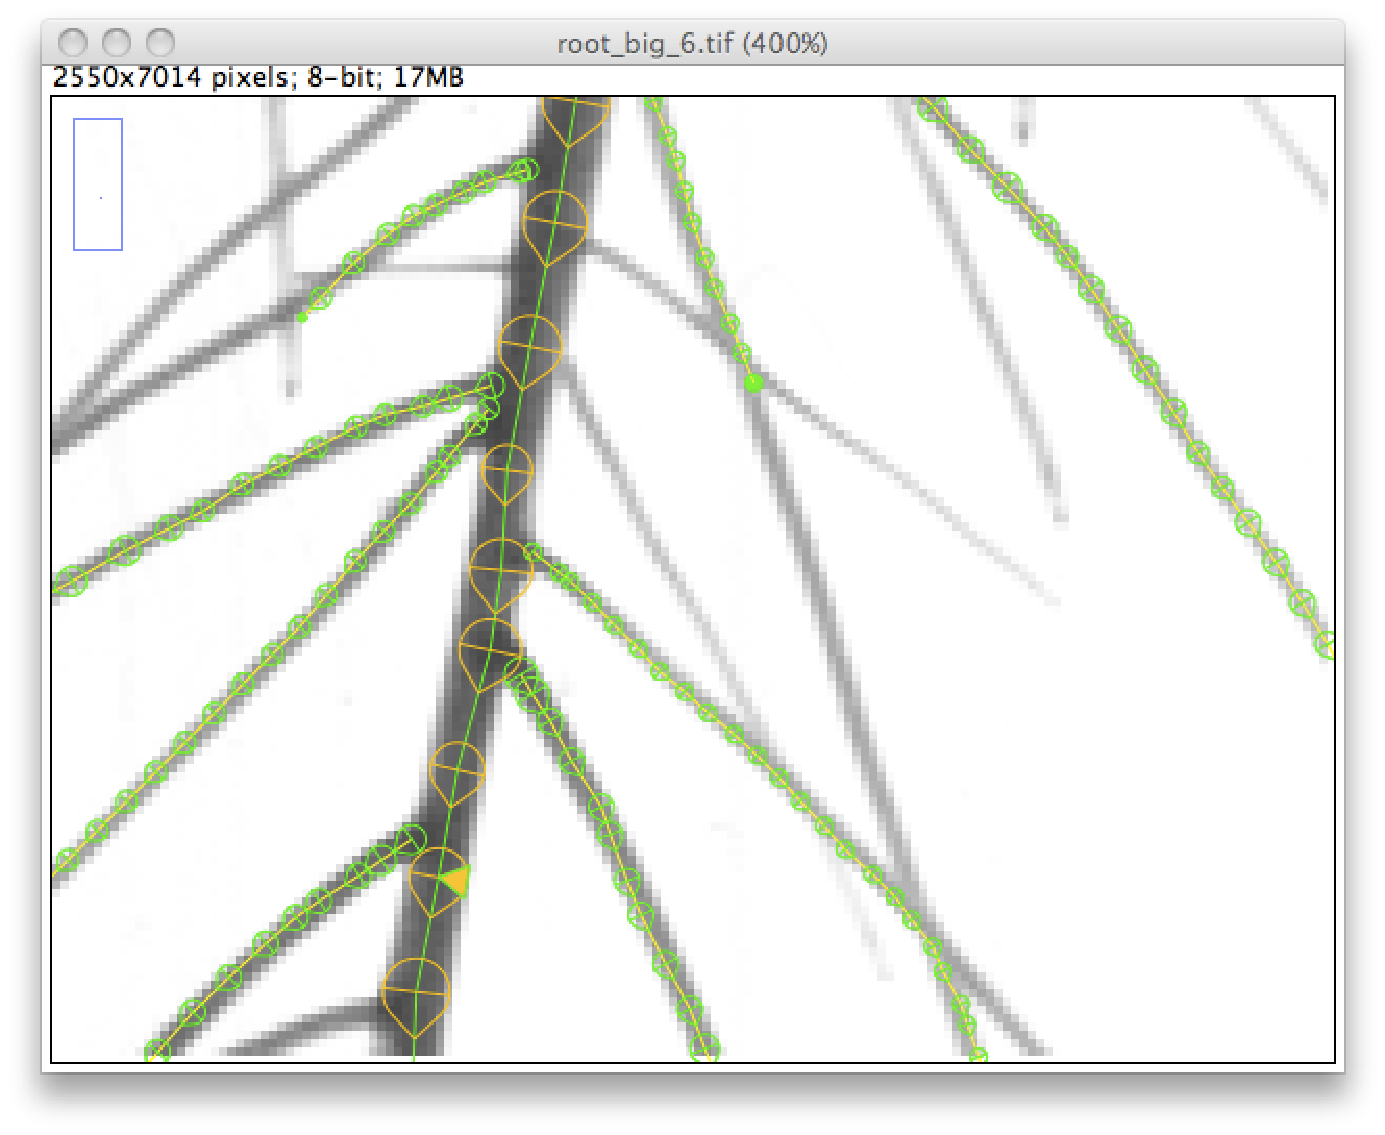
\includegraphics[width=7cm]{child1}
%\caption[Display of parent and children roots]{\textbf{Display of parent and children roots}: parent and children roots are displayed in different colors}
%\label{child1}
%\end{center}
%\end{figure}

In order to decrease to time needed a lateral finding algorithm was implemented in SmartRoot. To start the algorithm, right-click on a root and select \verb|Find laterals| (see sec. \ref{modify}). Settings of the algorithm could change from one image to the other. Information about the settings can be found in the section \ref{chapsettings}

%--------------------------------

\subsection{How to escape the \textit{centering} mechanism}

In semi-automatic tracing, SmartRoot detects situations where the root diameter suddenly increases by a given factor (by default 1.6) during the tracing. This typically happens when one reachs a region where the traced root comes so close to another root that it becomes virtually impossible to distinguish the two roots (fig. \ref{escape-1}).\\

When this happens, the diameter is prevented to increase and keeps the same value as that of the preceding node. As long as the next node diameter is more than 1.6 times that of the preceding node (possibly frozen) the correction will hold. In this situation, nodes are not anymore centered relative to the root object. Instead, they are aligned relative to the closest border of the root(s), at a distance corresponding to the root (frozen) radius (fig. \ref{escape-2}).\\

\begin{figure}[h]
\centering
   \subfloat[]{\label{escape-1}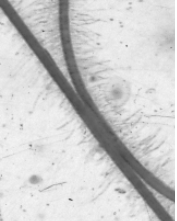
\includegraphics[width=2.5cm]{escape-1}}
  \hspace{10mm}   
  \subfloat[]{\label{escape-2}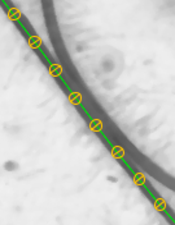
\includegraphics[width=2.5cm]{escape-2}}
\caption[Touching roots]{\textbf{Automatic tracing with touching roots}. (a) Two touching roots (b) Automatic drawing}
\label{2roots}
\end{figure}

The current implementation may fail in certain circumstances: if one of the roots is making too strong a bend, the algorithm may sweep to the other root, as illustrated on figure \ref{escape-3}.\\

\begin{figure}[h]
\centering
   \subfloat[]{\label{escape-3}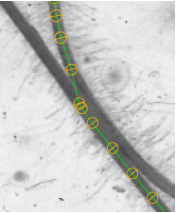
\includegraphics[width=2.5cm]{escape-3}}
  \hspace{10mm}   
  \subfloat[]{\label{escape-4}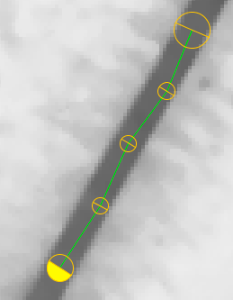
\includegraphics[width=2.5cm]{escape-4}}
\caption[Escape centering]{\textbf{Escape centering mechanism}. (a) Two touching roots (b) Automatic drawing}
\label{escape}
\end{figure}

When this occurs, the user will have to correct the tracing, typically by moving the first "bad" node to its correct position, clicking the \verb|Alt| key to tell SmartRoot to rebuild the root from there.\\

For this reason, the user is left the possibility to request the "diameter freeze" and "align to border" manually. To force the diameter of the current node to be equal to that of the previous node, just hold the control key while adding or moving the node (in this case, the node is placed at the exact position of the mouse). To force the current node to be aligned relative to the closest root border instead of to the root center, just hold the shift key while adding or moving the node.\\

The \verb|shift|, \verb|control| and \verb|alt| keys can be combined in any way and their effects are additive. Typically, to correct the root of the last illustration, just move the first badly aligned node while holding the \verb|control|, \verb|shift| and \verb|alt| keys together: the \verb|control| key will make sure that the node diameter is correct, the \verb|shift| key will make sure that the node is aligned to a border and the \verb|alt| key will request that the rest of the root be re-traced automatically.\\

On figure \ref{escape-4} is another example of combinations of the shift and control keys. The top node is the first one, it uses the default centering mechanism. The second node was adjusted to the right border (\verb|shift| key). The third node was forced to have the same diameter as the previous one (\verb|control| key). The fourth node was forced to have the same diameter and to be aligned on a border (\verb|shift| + \verb|control| keys). the last node was traced without any modifier key.

%------------------------------------

%
% \subsection[The CrossHair tool]{The CrossHair tool: how to get point measurements}
% 
% When you select the CrossHair tool, a ruler line is traced along the root axis which is the closest to the mouse, orthogonal to the closest root axis and aligned on the mouse position. The name of that root is displayed next to the mouse pointer (the label may not be displayed if the pointer is too far from all roots) (fig. \ref{crosshair-1}). 
% 
% \begin{figure}[htbp]
%\begin{center}
%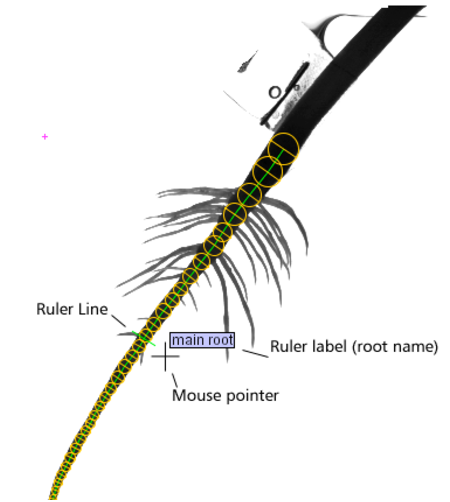
\includegraphics{crosshair-1}
%\caption[CrossHair tool]{\textbf{CrossHair tool}}
%\label{crosshair-1}
%\end{center}
%\end{figure}
% 
%When the mouse is clicked (with the crosshair tool), a number of measurements are calculated at the intersection between the root and the ruler line and are pasted in the SQL Vector window. These measurements are: the length of the root, the root diameter (at the ruler line intersection), the distance from the ruler line intersection to the root base ("LPOS" for Longitudinal POSition) and the angle (in radians) between the root axis (at the ruler line intersection) and the horizontal of the image (counted counter-clockwise). These data (along with the root name and image filename) can be exported to the ODBC datasource (\verb|Ctrl-w| for "Write") or to the system clipboard (the classical Ctrl-c). By default, SmartRoot assumes a 300DPI scanning resolution, but this setting can be modified (\verb|popup menu > Settings > Set DPI Value…|).\\
%
%The longitudinal position is calculated relative to some root origin which, by default, is the most proximal node of the root. While using the CrossHair or Mark tools, a different ruler origin can be chosen, by placing the ruler line at the desired location, raising the contextual popup menu (right click) and selecting "Set Ruler Origin". It is easy to see the effect of this when the Ruler is displayed (\verb|popup menu > Display options > show ruler|). The distances and length are given in centimetres. \\
%
%SmartRoot attempts to mirror the ruler line of the active window in any other image window which is opened at the same time. Whenever the ruler line tracks a root in the active window, SmartRoot starts looking for roots with the same name in all other opened window. When such roots are found, a "mirror" ruler line is displayed in the corresponding window at the same longitudinal position. This feature makes it easy to visually compare time series of root images (e.g. to match lateral roots at different time based on their longitudinal position along the parent root). It is particularly usefull with series of root images where the roots lay differently in successive images (ex. roots in hydroponics that are re-scanned every day). This feature is illustrated below with two images of the same root at 4 days interval.\\
% 
%  \begin{figure}[htbp]
%\begin{center}
%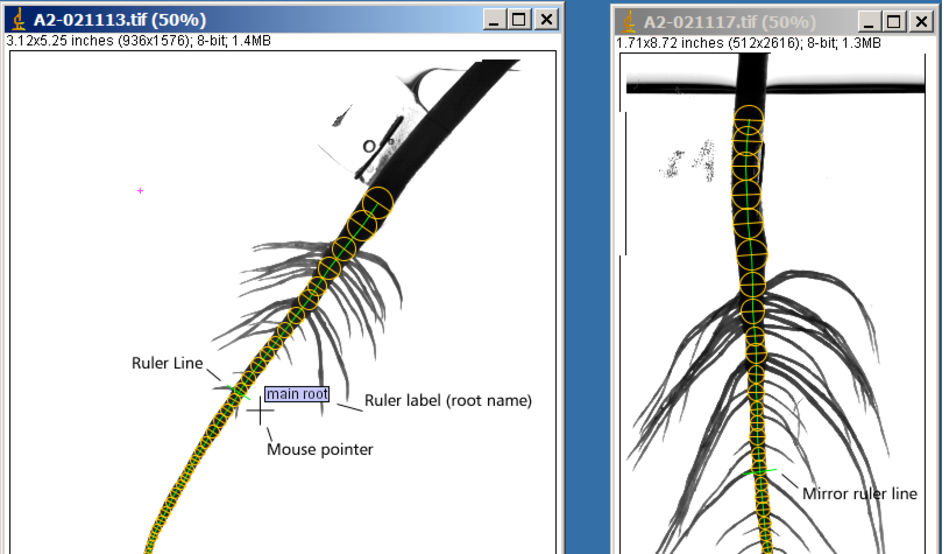
\includegraphics[width=13cm]{crosshair-2}
%\caption[CrossHair tool synchronised]{\textbf{CrossHair tool in synchronised windows}}
%\label{crosshair-2}
%\end{center}
%\end{figure}
% 
%It is also possible to force other (displayed) windows to focus on the same region than the visible region of the active window (fig. \ref{crosshair-2}). In ruler mode, the \verb|Synchronize other windows| item of the popup menu attempts to recenter any other root image window on the root object and at the longitudinal position corresponding to the root object intersected by the ruler line in the active window, and applies to all windows the same zooming factor as that of the active window.\\


%------------------------------------
\newpage
{\color{coolSection}\section[The Mark tool]{The Mark tool: how to annotate roots and get all measurements at once}}
\label{chapmark}

When you select the \verb|Mark| tool, a ruler line appears along the root axis which is the closest to the mouse, orthogonal to the closest root axis and aligned on the mouse position. The name of that root is displayed next to the mouse pointer (the label may not be displayed if the pointer is too far from all roots). A left-click will place a mark at this position. Marks are tools to enrich the information stored in the image and that can be exported. When adding a mark, the user will be asked to choose the kind of mark he wants to add. Indeed, several kind exist, depending of the kind of information you want to add to the image.\\

\begin{description}

\item [Free Text.] A single mark with a text field to annotate a specific point on a root (e.g. broken root, unexpected curvature, ...).

\item [Number.] A single mark with a number field to annotate a specific point on a root (e.g a date for time series, …). If other Number marks are present on the root, the default value proposed for the mark will be set according to its longitudinal position on the root.

\item [Most distant lateral.] A mark indicating the position of the most distant lateral of a root. It is automatically updated whenever a more distant lateral is created.

\item [Interval.] Twin marks defining a region of the root presenting specific features (e.g. poorly branched, cluster roots, ...).

\item[Measure.] The simplest mark in SmartRoot, which take measurement at its position (e.g. root diameter, position on the axis, ...). 

\end{description}



{\color{coolSection}\section[The Registration Anchor tool]{The Registration Anchor tool: Image Registration}}
\label{chapreg}

When working with time series of images of root system grown in solid substrates, it can be assumed that a root at time t will occupy the same 2D location at time t+1. In principle, it should therefore be possible to re-use every root object traced at time t on the image at time t+1 and, therefore, to avoid retracing the same roots for every image. Then, tracing the growth increment would simply require an \verb|Alt-click| (and short drag) on each root apex with the Trace tool (which will automatically construct the apical root segment grown between the two image acquisitions).\\

However, it is unlikely that the root material will be placed precisely at the same location relative to the scanner or camera on every images. This would result in small translation/rotation/rescaling of the roots when comparing two different images. The correction of these modifications is the object of image registration and is based on registration anchor points that are precisely located on the two images and that can be used to estimate the parameters of the translation/rotation/scaling transforms.\\

The implementation of Image Registration in SmartRoot assumes that the plane of the scanner/camera is always parallel to that of the root material, so it only needs two registration anchors. Working with Image Registration in SmartRoot involves the following steps:\\

\begin{enumerate}
\item In the image at time t (in which a number of roots have been traced), locate two image features (typically far from each other) that can be easily located on the image at time t+1. Point the Registration Anchor tool to the first feature and raise the popup menu to select "Add Registration Anchor". Repeat with the second feature and close the datafile. The registration anchors are stored in the datafile.
\item Open the image at time t+1 (it should have an empty datafile), locate the same two features and add the two registration anchors (as in 1.). Then select popup>File>Import Seed Datafile and select the xml file of image t. All root objects of image t should appear at the right place (i.e. correctly aligned on image t+1), but with the length and diameter they had at time t.
\item You will be prompted and asked if the tracing  and the roots are properly aligned. If not, press \verb|No| and replace the root by using the different arrows in the new window (fig. \ref{registration}). When the tracing is correctly placed, click \verb|OK|
\item Process to root tracing of the root growth increments and new roots.\\
\end{enumerate}


\begin{figure}[htbp]
\begin{center}
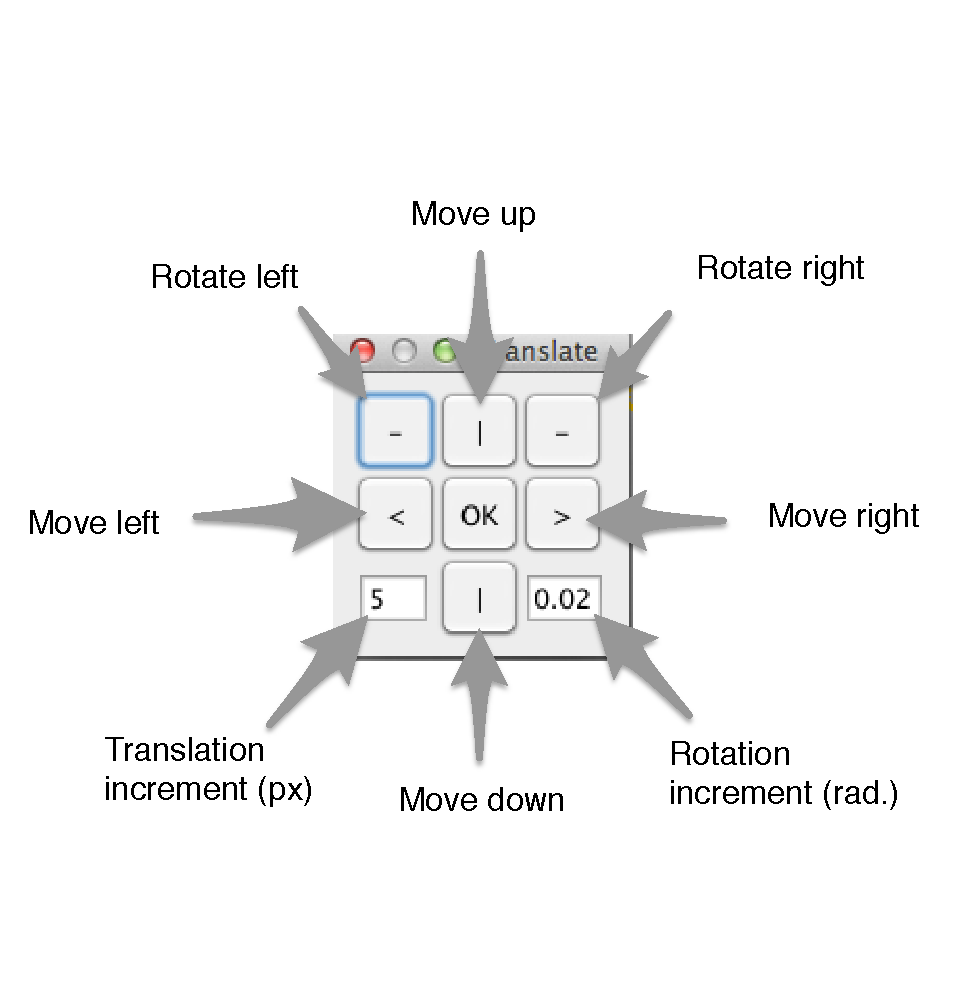
\includegraphics[width=0.7\linewidth]{registration}
\caption[Registration window]{\textbf{Registration window}}
\label{registration}
\end{center}
\end{figure}


%%%%%%%%%%%%%%%%%%%%%%%%%%%%%%%%%%%%%%%%%%%%%
%%%%%%%%%%%%%%%%%%%%%%%%%%%%%%%%%%%%%%%%%%%%%
%%%%%%%%%%%%%%%%%%%%%%%%%%%%%%%%%%%%%%%%%%%%%


\chapter{SmartRoot window tabs} 
\label{tabs}

{\color{coolSection}\section{Layers }}
\label{chapdisp}

The \verb|Layout| tab ing the SmartRoot window allows to select the root objects attributes that are displayed on top of the image (fig. \ref{display}). The \verb|Save in Prefs| stores the current selections so that they automatically apply when opening an image. The preferences are user-specific.
 
 \begin{figure}[!h]
\centering
  \subfloat[Nothing]{\label{disp-1}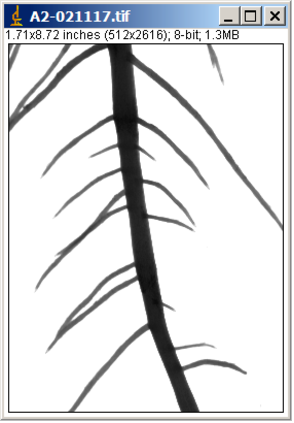
\includegraphics[width=3cm]{disp-1}}
  \hspace{5mm}   
  \subfloat[Display Axis]{\label{disp-2}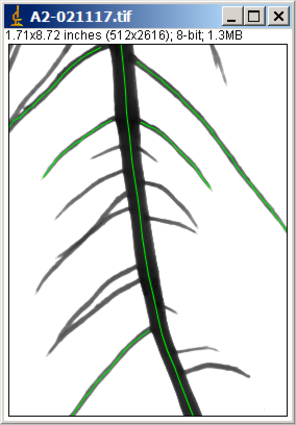
\includegraphics[width=3cm]{disp-2}}
  \hspace{5mm} 
  \subfloat[Display Nodes]{\label{disp-3}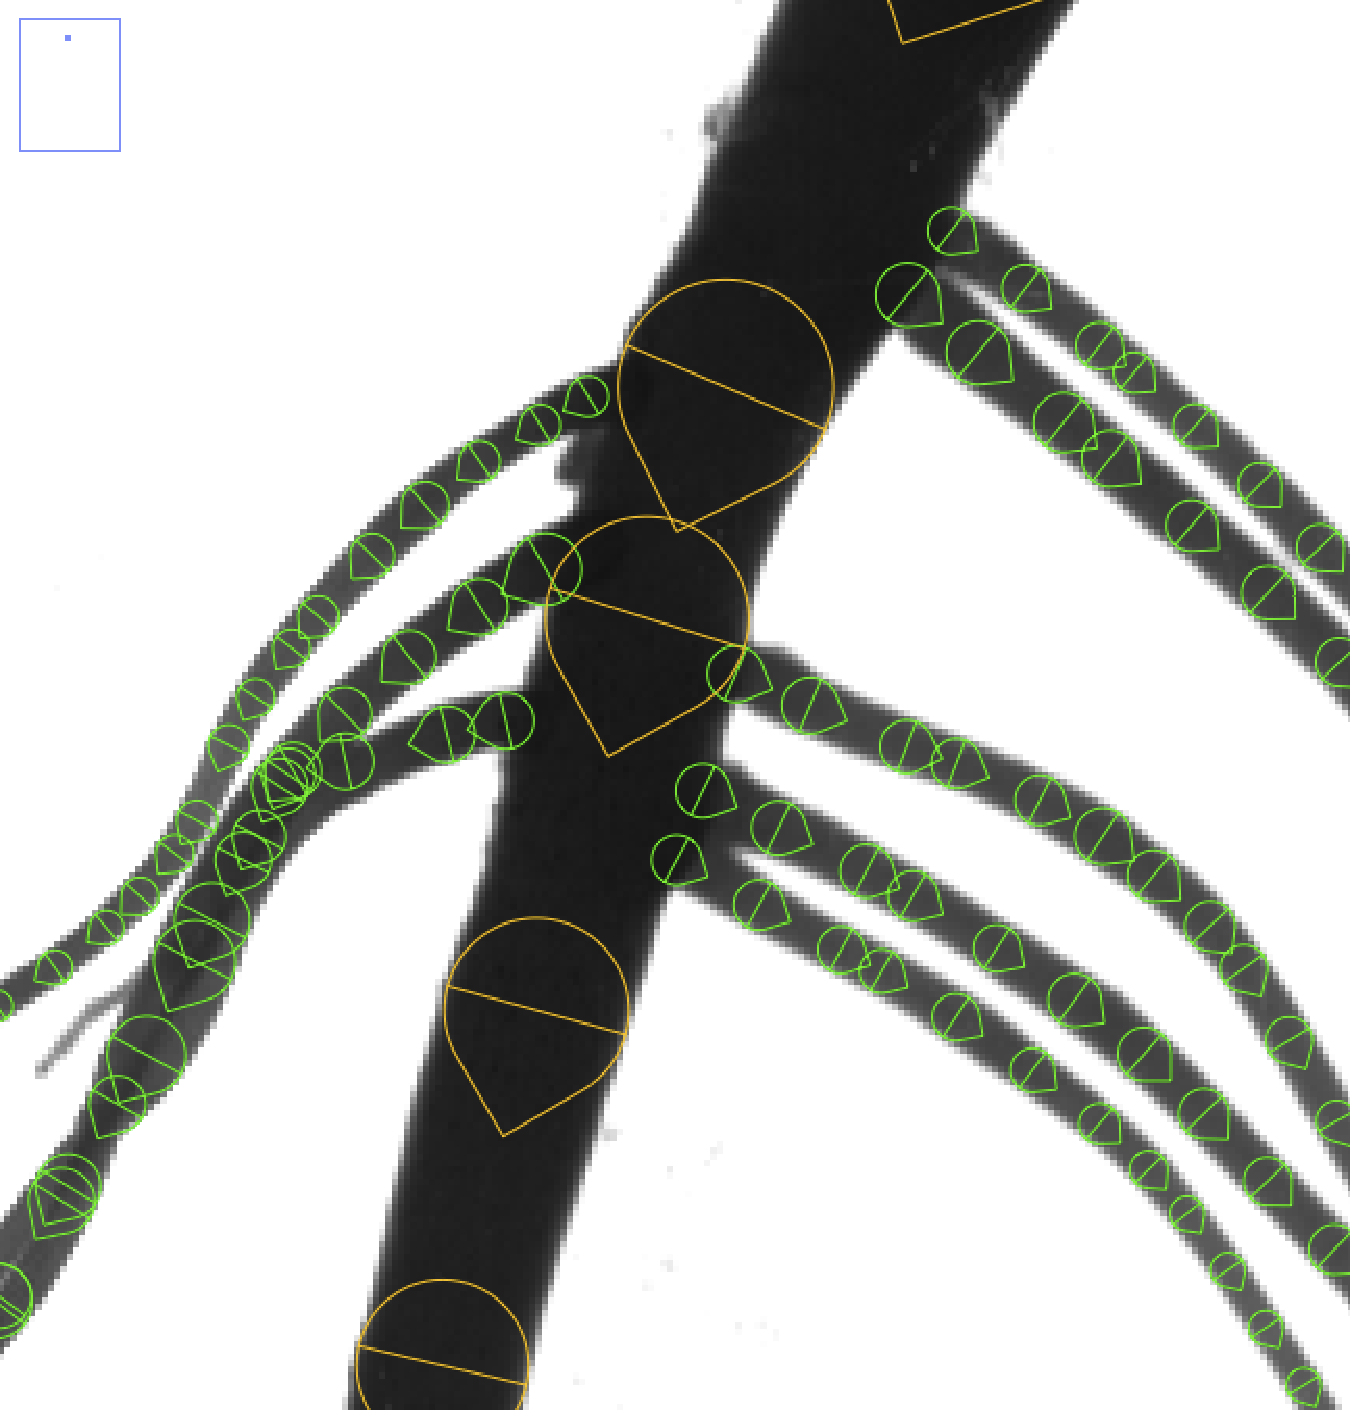
\includegraphics[width=3cm]{disp-3}}
  \hspace{5mm} \\
  \subfloat[Display Borders]{\label{disp-4}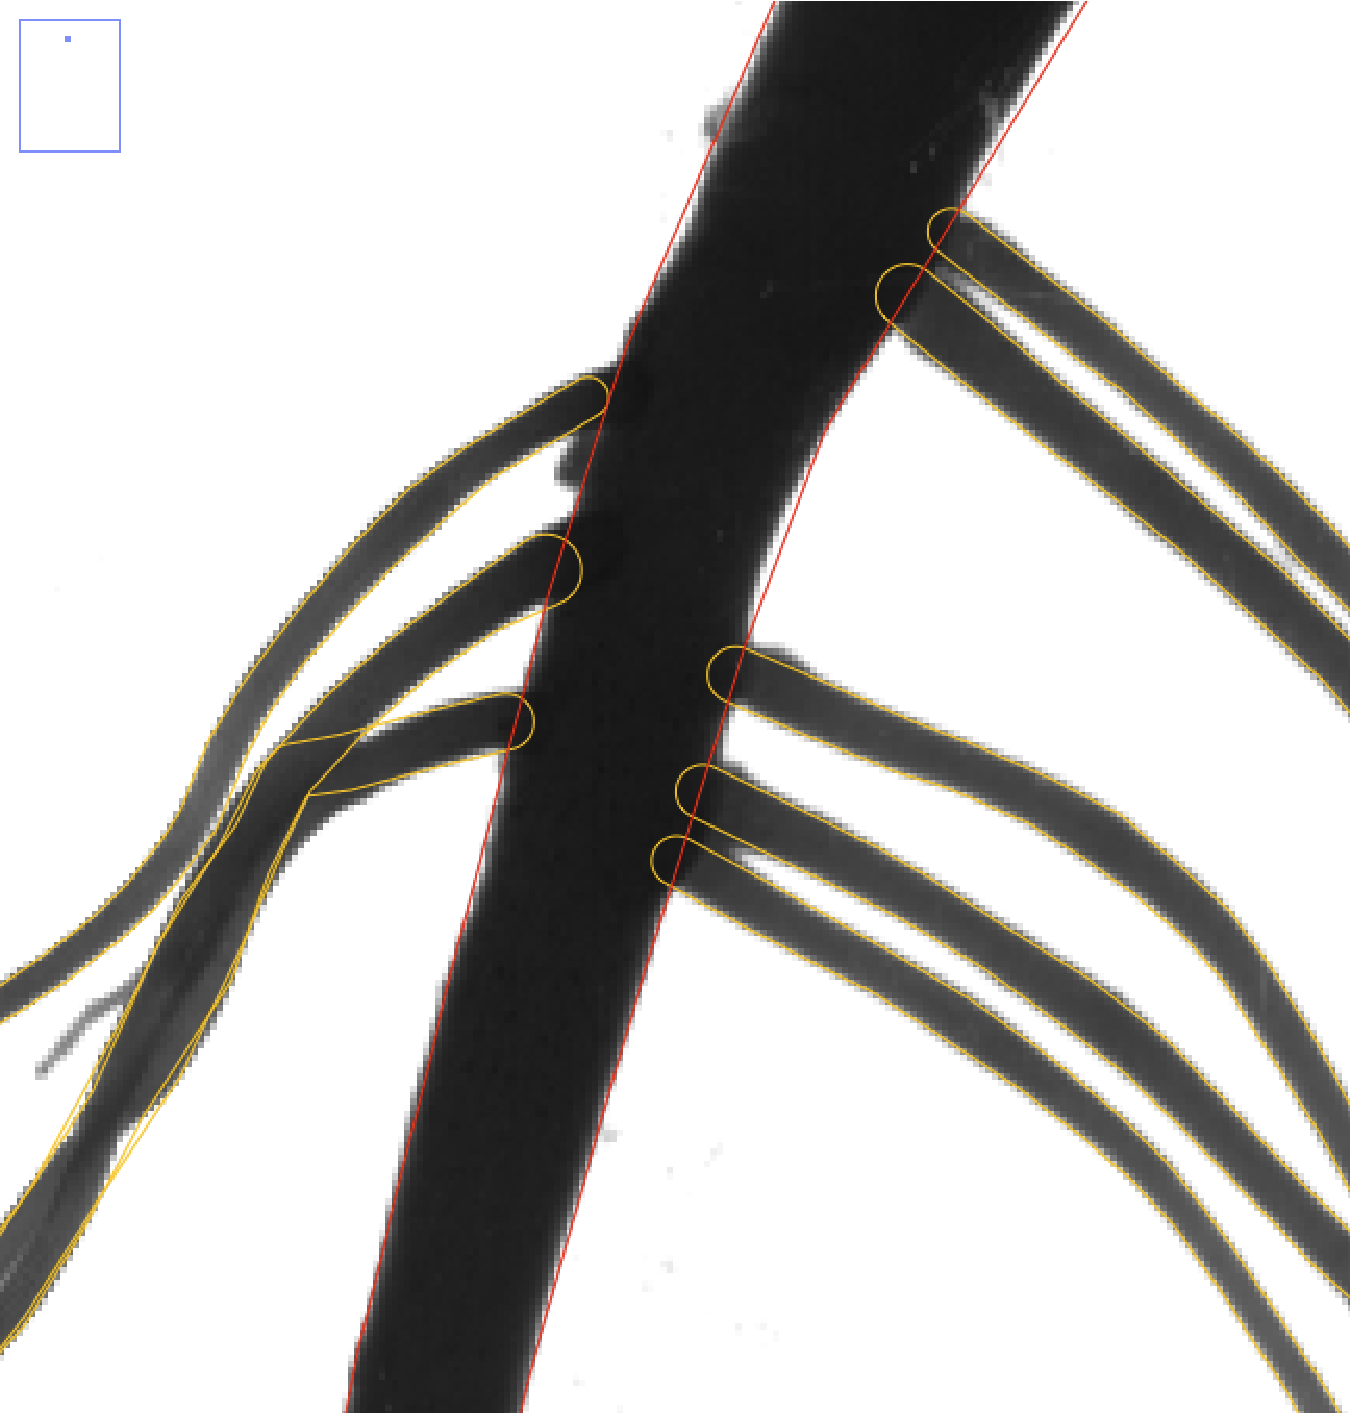
\includegraphics[width=3cm]{disp-4}}
  \hspace{5mm} 
  \subfloat[Display Area]{\label{disp-5}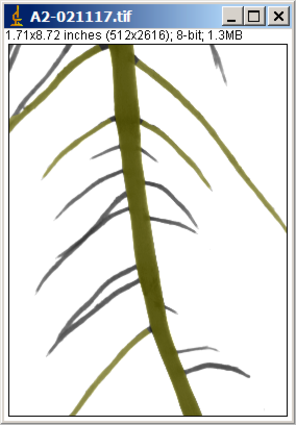
\includegraphics[width=3cm]{disp-5}}
  \hspace{5mm} 
  \subfloat[Display Ruler (and Axis)]{\label{disp-6}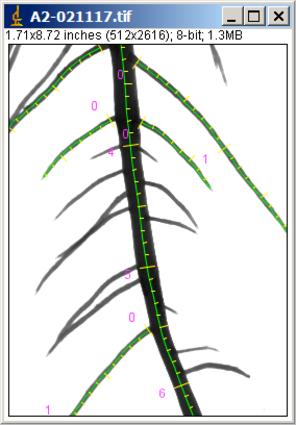
\includegraphics[width=3cm]{disp-6}}
  
\caption[Display options]{\textbf{Display options}.}
\label{display}
\end{figure}

%------------------------------------
\newpage
{\color{coolSection}\section{Root list}}
\label{chaprootlist}

The "Root list" tab of the SmartRoot window is divided in three panels. The upper left panel presents all the drawn root of the image as a tree (fig. \ref{rootlist} A and B) while the upper right panel display informations about the root selected in the tree (fig. \ref{rootlist} C). The bottom panel show all the marks of the selected root (ig. \ref{rootlist} D).\\

The selected root(s) will also appear in red on the image.\\

\begin{SCfigure}[][h]
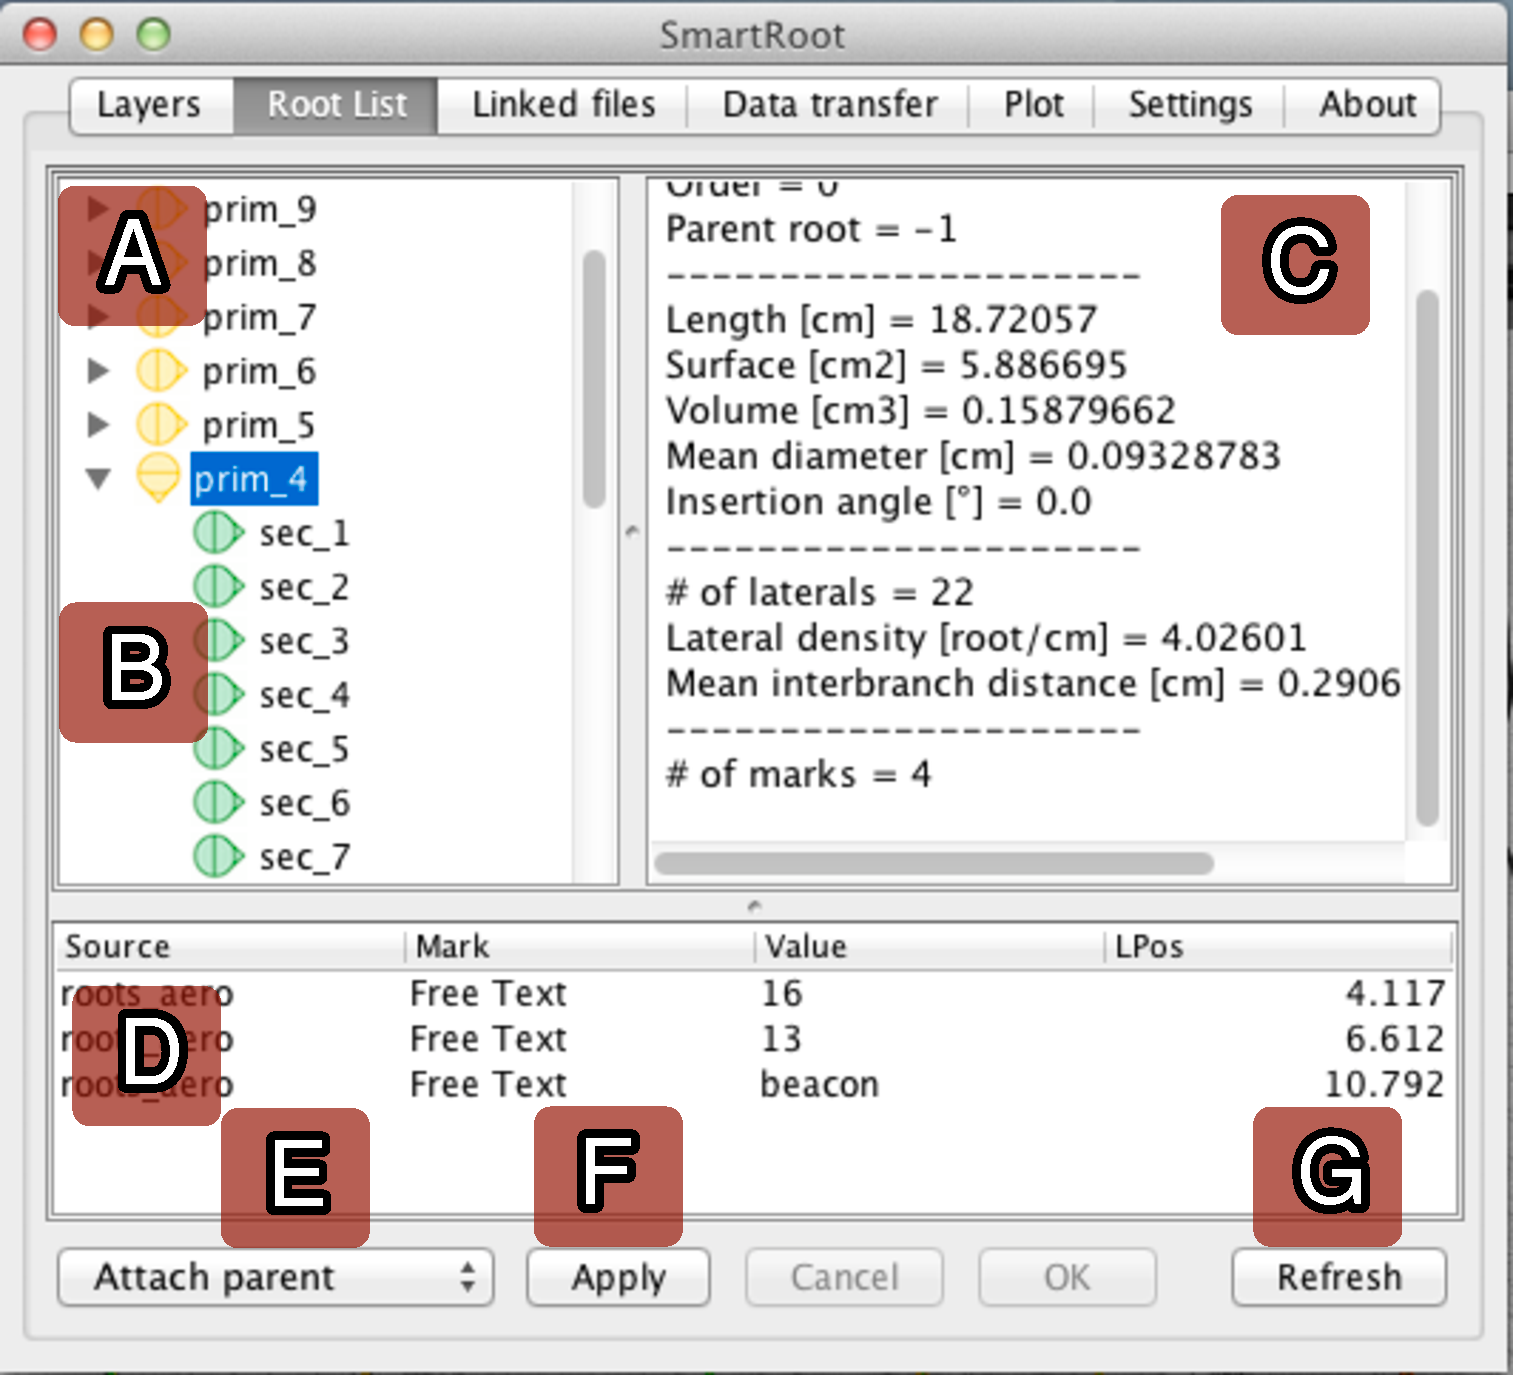
\includegraphics[width=0.6\linewidth]{root_list}
\caption[Root list]{\textbf{Root list}. 
\\ \\ \textbf{A} List of primary roots shown in yellow.\\ \textbf{B} If a root has children, they will be shown in green.\\ \textbf{C} The right shows information about the selected root(s). \\ \textbf{D} The bottom panel shows the marks of the selected root.\\ \textbf{E} Action menu to perform actions on the selected root(s).\\ \textbf{F} Apply button to validate the action chosen.\\ \textbf{G} Refresh button to refresh the root list (not done automatically)}
\label{rootlist}
\end{SCfigure}

\vspace{20pt}
This view allow the user to visualize easily the different root of the image as well as perform some action on them with the \verb|Action| button (fig. \ref{rootlist} E):

\begin{description}

\item [Delete root(s)] Delete the selected root(s). Can be performed on multiple items.

\item [Delete mark(s)] Delete the selected mark(s). Can be performed on multiple items.

\item [Rename root] Rename the selected root. Can be performed on only one item. Can also be done by double clicking on the root in the tree.

\item [Attach parent] Attach a new parent to the selected root(s). The user will be asked to selected the parent in the list and then click the "OK" button to validate his choice. Can be performed on multiple items.

\item[Detach parent] Detach the parent(s) of the selected root(s). Can be performed on multiple items. 

\item[Detach child(ren)] Detach the child(ren) of the selected root(s). Can be performed on multiple items. 

\item[Find laterals] Run the "Find lateral" function (see sec. \ref{modify}) on the selected root(s). Can be performed on multiple items. 

\end{description}
%--------------------------------------


\newpage

{\color{coolSection}\section{Linked files}}
\label{chaplink}

SmartRoot enables time-series analysis of root images. General principle is to trace the root you want to follow on every image of the time-series and to name them identically. Once the root of the last image is traced, click on the \verb|Linking files| panel of the \verb|SmartRoot| window. Then, choose the information you want to import on this last image (fig. \ref{SR-link}). All information will be displayed on the last image (fig. \ref{mark}) and  can therefore be exported to a single table in the database (see sec. \ref{chaptrans}).\\

 \begin{figure}[htbp]
\begin{center}
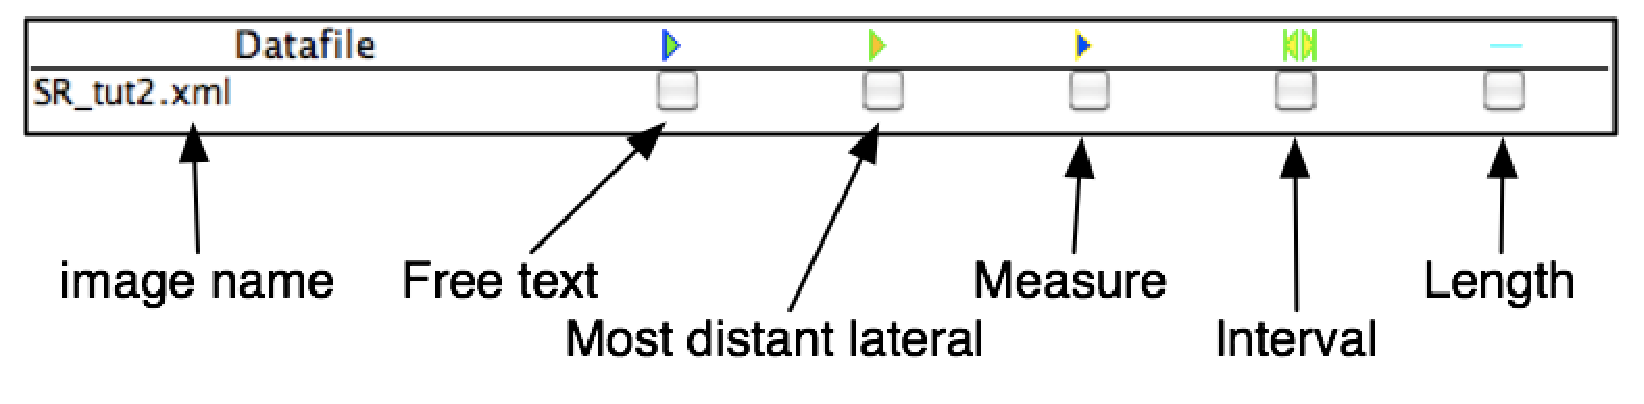
\includegraphics[width=12cm]{SR-link-tab}
\caption[Linking file tab in the SR window]{\textbf{Linking file tab in the SR window}:  this tab allows the user to import information from previously treated images on the current one}
\label{SR-link}
\end{center}
\end{figure}

 \begin{figure}[htbp]
\begin{center}
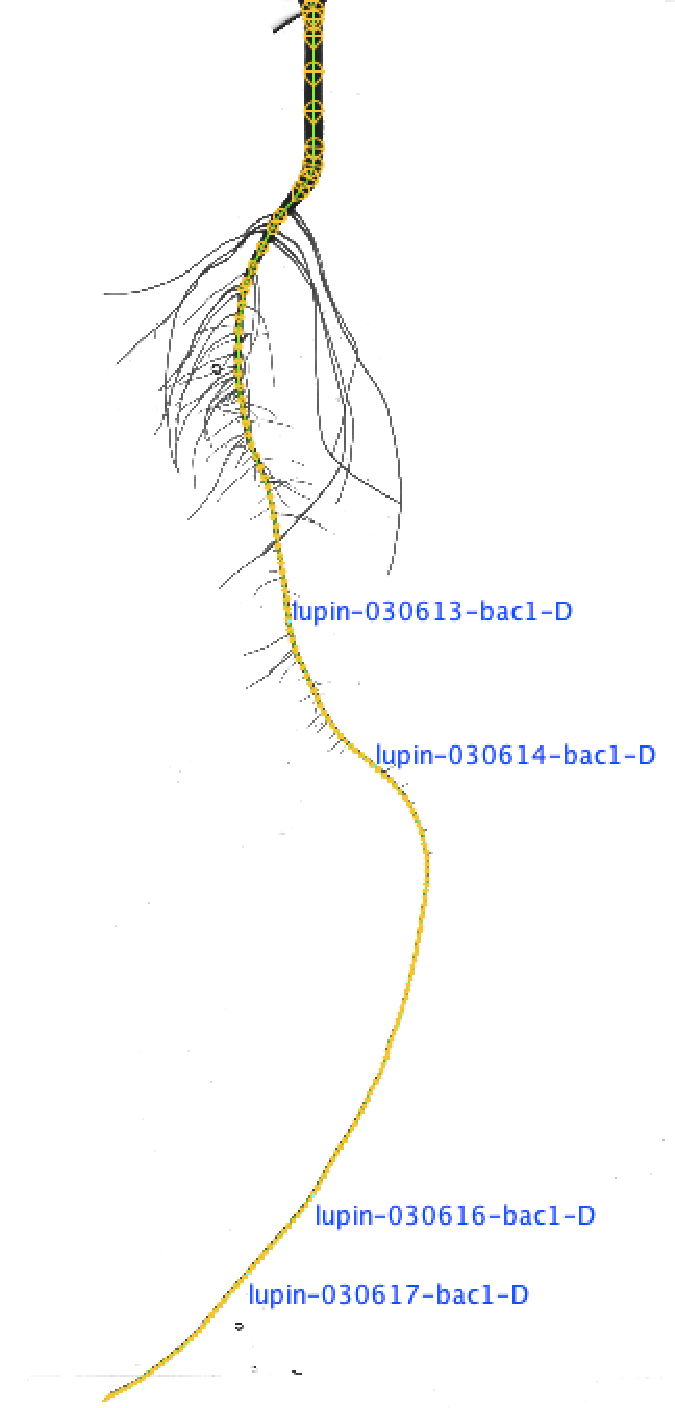
\includegraphics[width=5.5cm]{SR-link}
\caption[Linking files in SR]{\textbf{Linking files in SR}:  All informations contained in the previous images of the same time-series are displayed on the last image.}
\label{SR-link}
\end{center}
\end{figure}


%--------------------------------------

\newpage
{\color{coolSection}\section{Data transfer}}
\label{chaptrans}

SmartRoot as the ability to export data directly to a database as well as to a text file. To export data the your database or a .csv file (for database setup, see sec. \ref{install}), select the \verb|Data transfers| tab in the SmartRoot window. \\

\subsection{Send to SQL database\\}

\begin{itemize}
\item Check the \verb|Send to SQL database| checkbox 
\item Select the SmartRoot dataset (for details on export functions, see table \ref{export})
\item Check the \verb|Create new table| checkbox if you want to create a new table in the database. If the table already exist it will be overwritten
\item Click the \verb|Transfer| button. Look at the Results window for comments on transfer execution.\\
\end{itemize}

\subsection{Send to CSV text file\\}

\begin{itemize}
\item Check the \verb|Send to CSV file| checkbox 
\item Select the SmartRoot dataset (for details on export functions, see table \ref{export})
\item Choose where you want to save the .csv file
\item Write the name of the file (without extension)
\item Click the \verb|Transfer| button. Look at the Results window for comments on transfer execution.\\
\end{itemize}

\subsection{Send to image file}

This export generates an image of the traced roots (only the skeleton).

\begin{itemize}
\item Check the \verb|Send tracing to image file| chekbox
\item Choose the image type (color of black and white)
\item Choose the image format (.png, .bmp, .jpg or .tiff)
\item Choose the line width for the tracing
\item Choose the folder where to save the image
\end{itemize}

\subsection{Batch export}

It is often the case that the tracing of all the images is done prior to the export of the data. This function allows the user to export all the data at the same time, without re-opening the already traced images. The function will gather the informations directly into the .xml datafiles without opening the images (hence making it faster to export).

\begin{itemize}
\item Choose the folder containing the traced images and their corresponding .xml datafiles.
\item Choose the export you want to use (SQL, CSV or image) and provide the needed informations accordingly (for more information see previous section).
\end{itemize}



\subsection{SmartRoot Datasets\\}

\noindent \textbf{Global Root Data:}\\ 
This export function provides information about individual roots .\\

\noindent \textbf{Root Nodes:\\} 
This export function provides information about individual nodes.\\

\noindent \textbf{All Marks:\\} 
This function provides function about all the marks of the image. additionally to the marks added by the user, SmartRoot export an \verb|Origin| mark (beginning of the root) and a \verb|Length| mark (end of the root). Diameter and angle measurement are taken at the mark position. Mark value depend on the type of mark (see sec. \ref{mark}).\\

\noindent \textbf{Root Length Density:\\} 
This export function is use for plants grown in flat boxes (rhizotrons). It measure to root length density (root cm / soil cm$^3$) in user defined area. You have to know the thickness of the rhizotron. When you choose this export function, a specific window will appear, in order to define the region you want to analyze (fig. \ref{rld}).\\

\begin{figure}[htbp]
\begin{center}
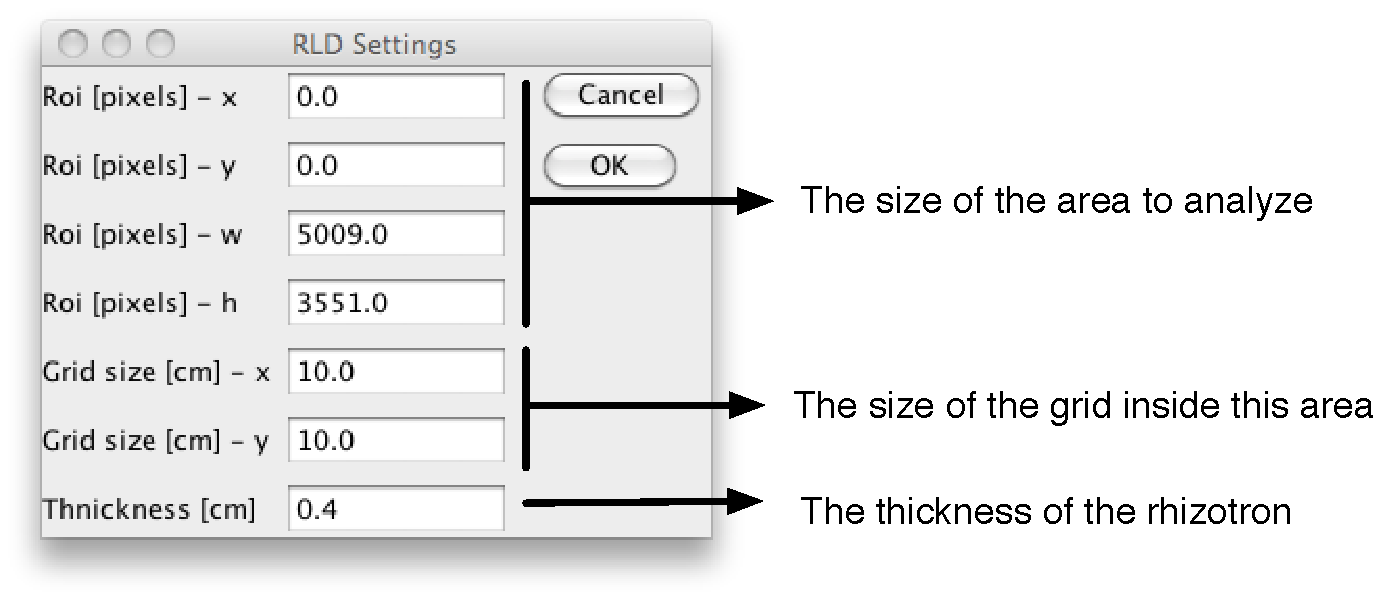
\includegraphics[width=10cm]{rld}
\caption[Root Length Density export settings]{\textbf{Root Length Density export settings}}
\label{rld}
\end{center}
\end{figure}

\noindent \textbf{Growth rate:\\} 
This export function is use for time lapse drawing of plants grown in flat boxes (see sect. \ref{root_growth}). It will export root growth based on the marks (Free text or Number) on the roots.\\


\begin{table}[!htdp]
\caption{Field explanation of the export functions in SmartRoot}
\begin{center}
\begin{tabular}{|lp{10cm}|}\hline 
Field Name & Description \\ \hline \hline

child\_density & number of children / cm of parent root in the ramified region \\ 
diameter  & root diameter (for a root, the mean diameter of all nodes)\\ 
first\_child  & identifier of the first child (from the base)\\ 
distance\_from\_base  & position of the node relative to the root base\\
distance\_from\_apex  & position of the node relative to the root apex\\
growth & growth since the last measure\\
image & image name\\
insertion\_angle & insertion angle on the parent\\
insertion\_first\_child  & position of the first child (from the base)\\
insertion\_last\_child & position of the last child (from the base)\\
insertion\_position  & insertion position on the parent (from the base)\\
last\_child  & name of the last child (from the base)\\
length  & root length\\
surface  & outer surface of a root, seen as a sequence of truncated cones\\
volume  & volume of a root, seen as a sequence of truncated cones\\
n\_child & number of children\\ 
parent  & parent identifier\\
root  & root identifier\\
root\_name  & root name\\
root\_ontology  & root type based on ontology classification\\
root\_order  & root ramification order (0 = first order root)\\
theta  & orientation of the node (radian) \\
value  & value of the mark (see table \ref{mark_val})\\
x  & x-coordinate (in cm) of the node center \\
y  & y-coordinate (in cm) of the node center \\ \hline

\end{tabular}
\end{center}
\label{mark_val}
\end{table}%

%
%
%\begin{table*}[!htdp]
%\caption{Field explanation of the export functions in SmartRoot}
%\begin{center}
%\begin{tabular}{|llp{7cm}|}\hline 
%Export options & Field Name & Description \\ \hline \hline
%\textbf{Global Root Data} & Img  & image name\\
%& Root  & root name\\
%& Length  & root length\\
%& Diam  & root mean diameter\\
%& rootOrder  & root ramification order\\
%& parent  & parent name\\
%& LPosParent  & insertion position on the parent\\
%& insertAng & insertion angle on the parent\\
% & nChild & number of children\\ 
%& childDensity & number of children / cm of parent root in the ramified region \\
%& firstChild  & name of the first child (from the base)\\
%& LPosFirstChild  & position of the first child (from the base)\\
% & lastChild  & name of the last child (from the base)\\
% & LPosLastChild & position of the last child (from the base)\\ \hline \hline
% 
%\textbf{Root Nodes} & Img  & image name\\
%& Root  & root name\\
%& X  & x-coordinate of the node center \\
%& Y  & y-coordinate of the node center \\
%& theta  & orientation of the node (radian) \\
%& Diam  & diameter of the node\\
%& bLength  & position of the node relative to the root base\\
%& aLength  & position of the node relative to the root apex\\
%& rootOrder  & ramification order of the root\\
%& insertA  & insertion point on the parent (from the base)\\
%& parentRoot  & name of the parent root\\ \hline \hline 
%
%\textbf{All Marks} & Img  & image name \\
%& Root  & root name\\
%& Mark  & type of mark\\
%& LPos  & longitudinal position of the mark\\
%& Diam  & diameter of the root at the mark position\\
%& Ang  & root orientation at the mark position\\
%& PosX  & x-coordinate of the node center\\
%& PosY  & y-coordinate of the node center\\
%& rootOrder  & ramification order of the root\\
%& Val  & value of the mark (see table \ref{mark_val})\\\hline \hline
%
%\textbf{Root Length Density} & Img & image name   \\
%& x  & x coordinate of the top left corner of the considered surface\\
%& y  & y coordinate of the top left corner of the considered surface\\
%& RLD & root length density in the considered surface \\ \hline \hline
%
%\textbf{Root Growth} & Img  & image name \\
%& Root  & root name\\
%& LPos  & longitudinal position of the mark\\
%& Ang  & root orientation at the mark position\\
%& PosX  & x-coordinate of the node center\\
%& PosY  & y-coordinate of the node center\\
%& rootOrder  & ramification order of the root\\
%& date & day of the measure\\
%& growth & growth since the last measure\\ \hline
%\end{tabular}
%\end{center}
%\label{export}
%\end{table*}%
%
%\begin{table}[htdp]
%\caption[Mark values]{Marks specific values for the different kind of marks}
%\begin{center}
%\begin{tabular}{ll} \hline
%Mark & Value\\ \hline \hline
%Most Distant Lateral & 0\\
%Interval & LPos of the twin mark\\
%Free Text & user defined text\\
%Measure & MEASURE\\
%Origin & image name\\ 
%Length & image name\\ \hline
%\end{tabular}
%\end{center}
%\label{mark_val}
%\end{table}%

\noindent
\fbox{\parbox{\linewidth}{
{\color{red}\textsc{Important:}}\\

If you check the 'Create new table' check box, a new table will be create in the database if none exist. If an other database with the exact same name existed while transferring, it will be erased. To add data to and existing table, uncheck this checkbox.\\}}
\\

\vspace{20pt}

When you choose the name of your table, you should follow certain rules to avoid SQL syntax errors. For instance use the character underscore (\verb|_|) instead of space and do not use accentuations. Certain words, such as \verb|table| are use in the database syntax and their use to name tables will result in errors. Complete list of forbidden names can be found on the following web page: \\

\vspace{20pt}

\noindent
%\begin{footnotesize}
\fbox{\parbox{\linewidth}{%
\textbf{MySQL:} \url{http://dev.mysql.com/doc/refman/5.5/en/reserved-words.html} \\
\textbf{Access:} \url{http://msdn.microsoft.com/en-us/library/aa238507\%28SQL.80\%29.aspx}}}\\ 
%\end{footnotesize}

%--------------------------------------

%\newpage
%{\color{coolSection}\section{Summary}}
%\label{chapSummary}
%
%In this tab of the SmartRoot window, the user can visualize global informations about the selected image such as the number of root (principal and laterals), the average diameter, insertion angle, length, etc (fig. \ref{summaryfig}).
%
%
%  \begin{figure}[htbp]
%\begin{center}
%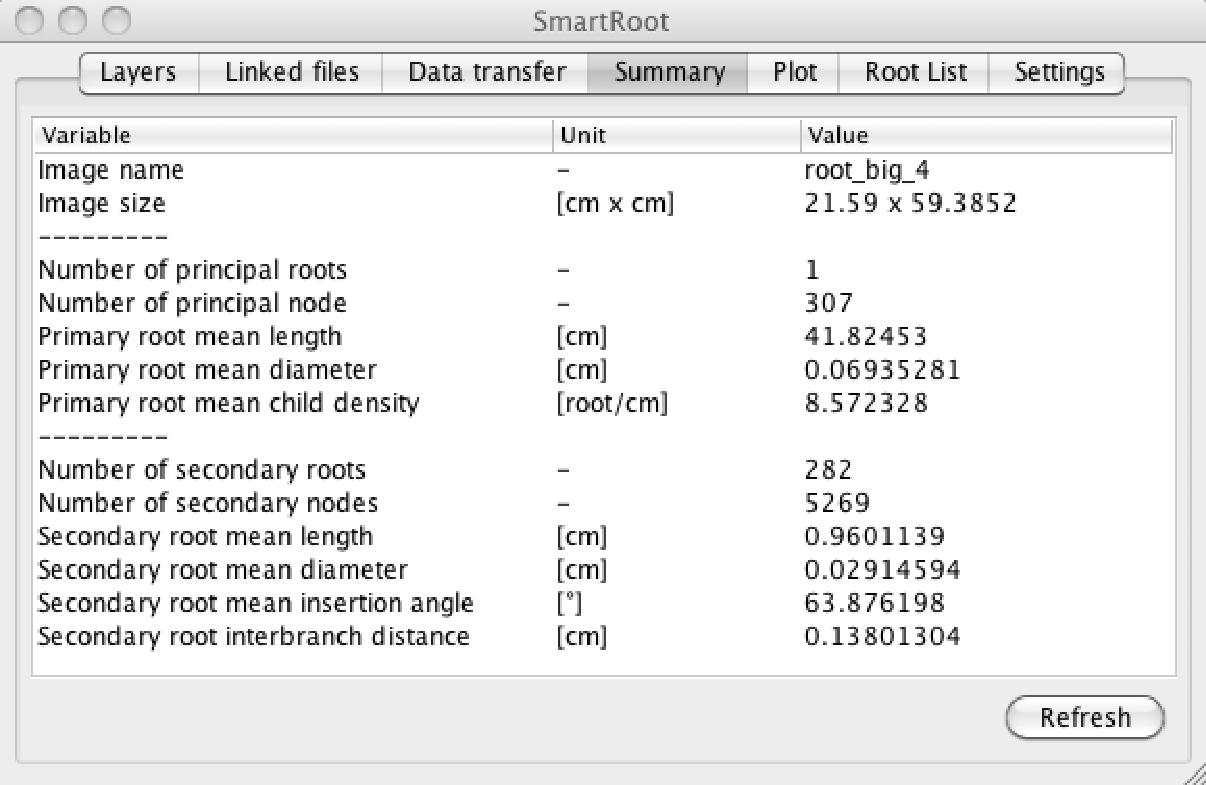
\includegraphics[width=10cm]{summary}
%\caption[Summary tab]{\textbf{Summary tab}:  this tab of the Smartroot window allows the user to visualize some global data about the current image.}
%\label{summaryfig}
%\end{center}
%\end{figure}

%--------------------------------------

\newpage
{\color{coolSection}\section{Plot}}
\label{chapplot}

In the SmartRoot windows, the user can choose the \verb|Plot| tab to access the build-in plotting capabilities of SmartRoot. The aim of this tools is not to provide a first analysis of the data, but rather a rough insight. The figure \ref{plot} shows plotting examples.\\

%\begin{SCfigure}[][htbp]
%\centering
%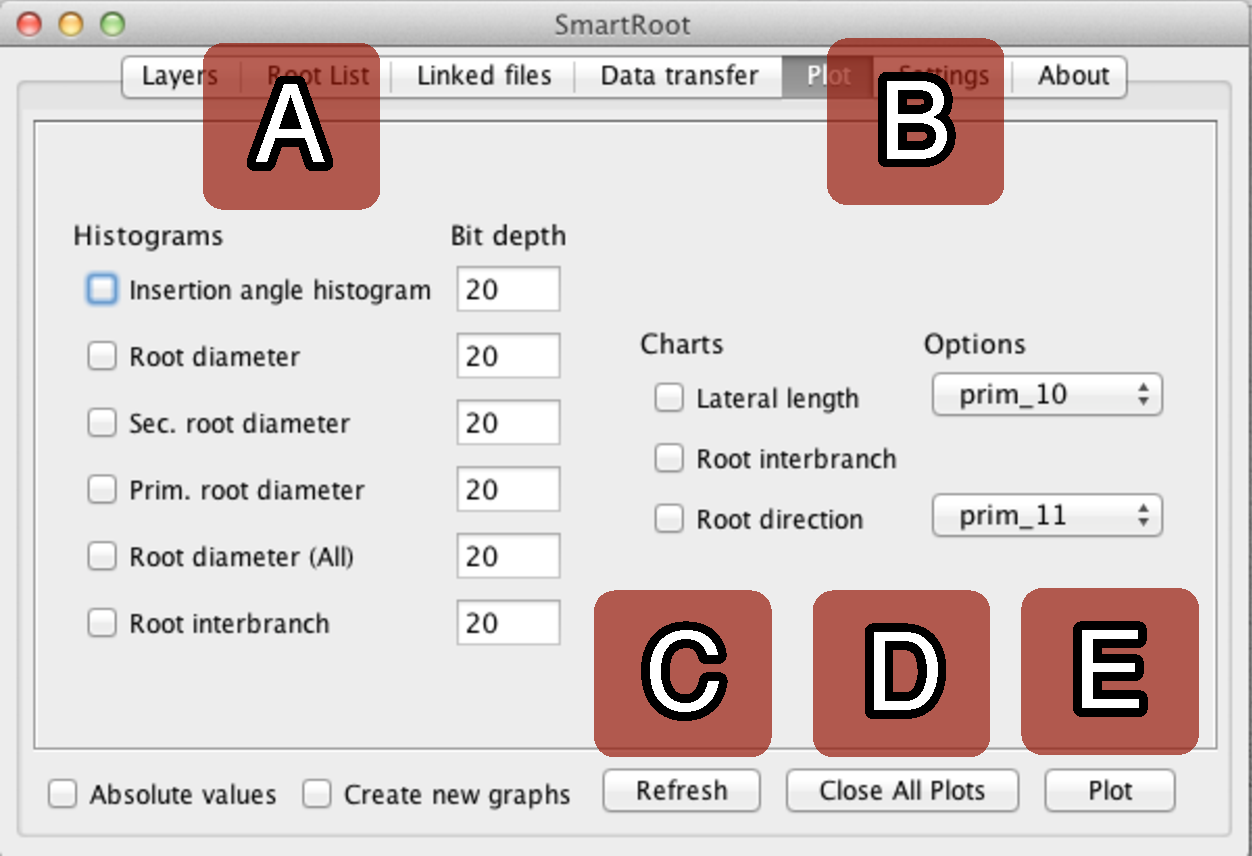
\includegraphics[width=0.5\linewidth]{SR_plot}
%\caption[Plotting examples]{\textbf{Plot Tab}\vspace{10pt}\\  
%\textbf{A} Histograms\\
%\textbf{B} Charts\\
%\textbf{C} Refresh button. Used to refresh the root lists\\
%\textbf{D} Close all plots.\\
%\textbf{E} Plot the selected charts and histograms}
%\label{SR_plot}
%\end{SCfigure}

\subsection{Histograms\\}
\label{hist}

Several types of histograms can be created such as the distribution of root diameter (for difference ramification orders), root insertion angles, or root inter-branch distance (the distance between two laterals). The number of classes of the histogram can be set by the user int he \verb|bits| field. The default unit of histograms is frequencies but it can be set to absolute values by selecting the \verb|Absolute value| checkbox.

\subsection{Charts\\}
\label{chart}

Three kind of charts can be generated inside SmartRoot: 

\begin{itemize}
\item inter-branch distance vs position on parent axis
\item lateral root length vs position on parent axis
\item change in direction vs position on the root (only for root of ramification order 0)
\end{itemize}

As these charts are generated with the information of single root, you will have to select the root you want the plot. To do so, click the \verb|Refresh| button to actualize the root of the current image. Then choose the wanted root in the root list (under \verb|option|). The selected root will appears in red on the image (if you check the corresponding checkbox).\\

  \begin{figure}[htbp]
\begin{center}
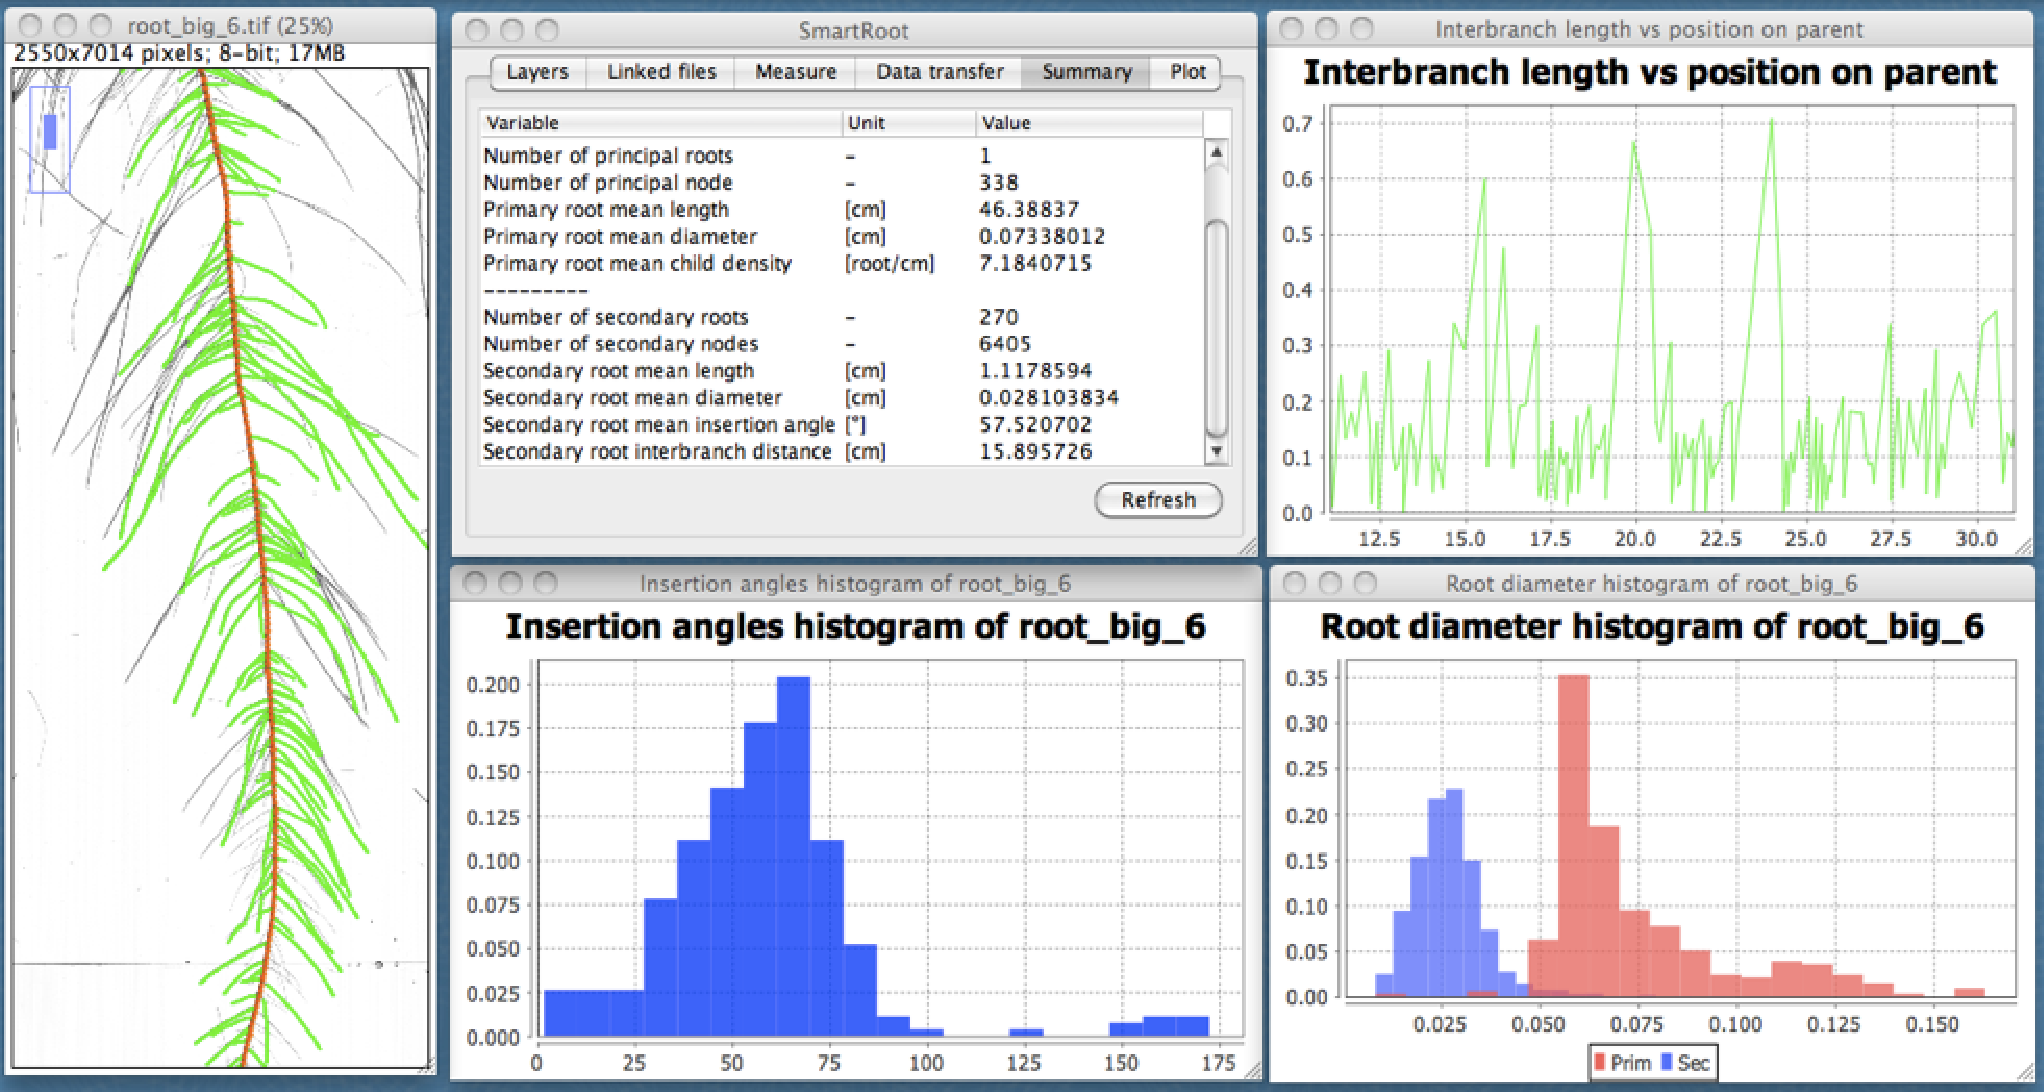
\includegraphics[width=14cm]{plot}
\caption[Plotting examples]{\textbf{Plotting examples}:  on this figure we can see a two histograms (of the insertion angles of laterals and of root diameter per order) and a chart of the inter-branch distance along the parent root axis.}
\label{plot}
\end{center}
\end{figure}

%--------------------------------------


\newpage
{\color{coolSection}\section{Settings}}
\label{chapsettings}

\subsection{Image resolution}  
\label{resolution_options}

SmartRoot allow the user to set the image resolution based on the DPI value of the image or a random value based on a scale visible on the image. 

To use a scale on the image, simply draw a line on the scale, click the \verb|Get Line| button and set the physical length of the scale. The unit can be chosen between cm, mm and inch. Click the \verb|Apply| button to set the scale on the image. SmartRoot will use either the DPI or the cm/mm/inch value based on the box you checked. 

The default value for the scale is the one stored within the image. This default value will not be used once you saved an image with SmartRoot. SmartRoot will use the value stored in the .xml file linked with the image.

Click the \verb|Set as default| button to set the current DPI value as the default DPI value for all the newly opened images.

\subsection{Naming options}
\label{name_options}

Once you draw a root SmartRoot choose a new name for it. The software will use a prefix and a sequential number based on the number of root already traced in the image. 

The prefix of the root names can be changed by the user. The \verb|Principal root prefix| applies for the root traced manually or with the line-drawing utility. The \verb|Lateral root prefix| applies for the lateral roots traced with the \verb|Find laterals| function. 

If the \verb|Ask for name| box is checked, the user will be ask to confirm the root name every time a new root is traced. 

\subsection{SQL options}
\label{sql_options}

These options are used to connect SmartRoot to the database. There are optional if you choose to use the CSV export. See section \ref{install} for details on how to setup the database depending on your operating system.


\subsection{Lateral research parameters}
\label{lat_options} 

The \verb|Find lateral| function use several test while building the new laterals. These tests can be disabled or parametrized depending on the image type and / or quality.

\begin{description}
\item[Number of steps along the root] Number step between two node while screening parallels of the selected root. The bigger is the number, the bigger is the precision but the longer is the research.
\item[Check the size of the nodes] If selected, the algorithm will check the diameter of the base node of every newly created laterals. If the node is either too big or too small, the root will not be created. This size is relative to the diameter of the parent node. A size of 1 means a size equal to the parent node's
	\begin{description}
	\item[Minimal diameter of a node] Define the minimal size of the node. 
	\item[Maximal diameter of a node] Define the maximal size of the node.
	\end{description}
\item[Check the size of the roots] Check the size of newly created root. If this root is too small, it is considered as noise and is deleted.
	\begin{description}
	\item[Minimal size of a lateral] Define the minimal size of the newly created root. This size is relative to the diameter of the parent node. A size of 1 means a size equal to the parent node's.
	\end{description}
\item[Check the direction of a node] Check the insertion angle of the newly created root. Force to root to be created in a given direction
	\begin{description}
	\item[Maximal insertion angle] Define the maximal insertion angle possible for a newly created lateral root.
	\end{description}
\end{description}

\subsection{Thresholding method} 
\label{th_options}

The thresholding method used by SmartRoot can be chosen between an \verb|Adaptive thresholding| method or a fixed threshold based on ImageJ threshold. It is recommended to used the \verb|Adaptive thresholding| for optimal performances.


%--------------------------------------

%%%%%%%%%%%%%%%%%%%%%%%%%%%%%%%%%%%%%%%%%%%%%
%%%%%%%%%%%%%%%%%%%%%%%%%%%%%%%%%%%%%%%%%%%%%
%%%%%%%%%%%%%%%%%%%%%%%%%%%%%%%%%%%%%%%%%%%%%


\chapter{Miscellaneous informations}


{\color{coolSection}\section{Root growth measurement in rhizotrons}}
\label{root_growth}

Growing plant in rhizotrons is an easy way to track root growth over time:

\begin{itemize}
\item simply place a transparent sheet on the transparent surface of the rhizotron
\item draw the root seen on the surface.
\item write the day at the apex position (fig. \ref{root_growth_drawing}).
\item come back on a regular basis and repeat the process by appending new tracing to the old ones
\end{itemize}

\begin{figure}[htbp]
\begin{center}
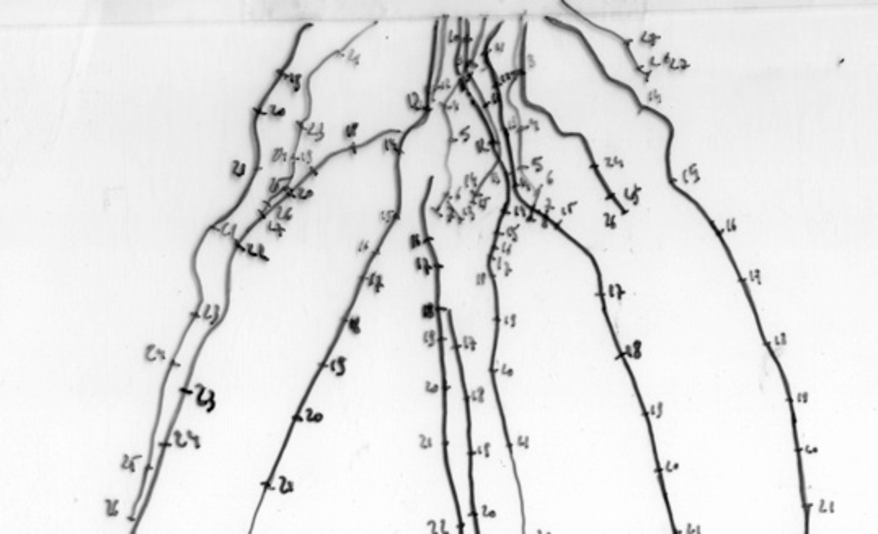
\includegraphics[width=10cm]{root_growth_drawing.pdf}
\caption[Root growth drawing]{\textbf{Example of hand drawing of root growth on a rhizotron surface}}
\label{root_growth_drawing}
\end{center}
\end{figure}

Once the tracing is done, you will have to process it in SmartRoot as follows:

\begin{itemize}
\item trace the different roots, with topology if necessary
\item us the Mark tool to place Free Text mark were you point the apexes
\item set the value of the mark to the day on which you trace the apex (fig. \ref{root_growth_drawing_close})
\item use the export function "Root Growth" and you are done
\end{itemize}

\begin{figure}[htbp]
\begin{center}
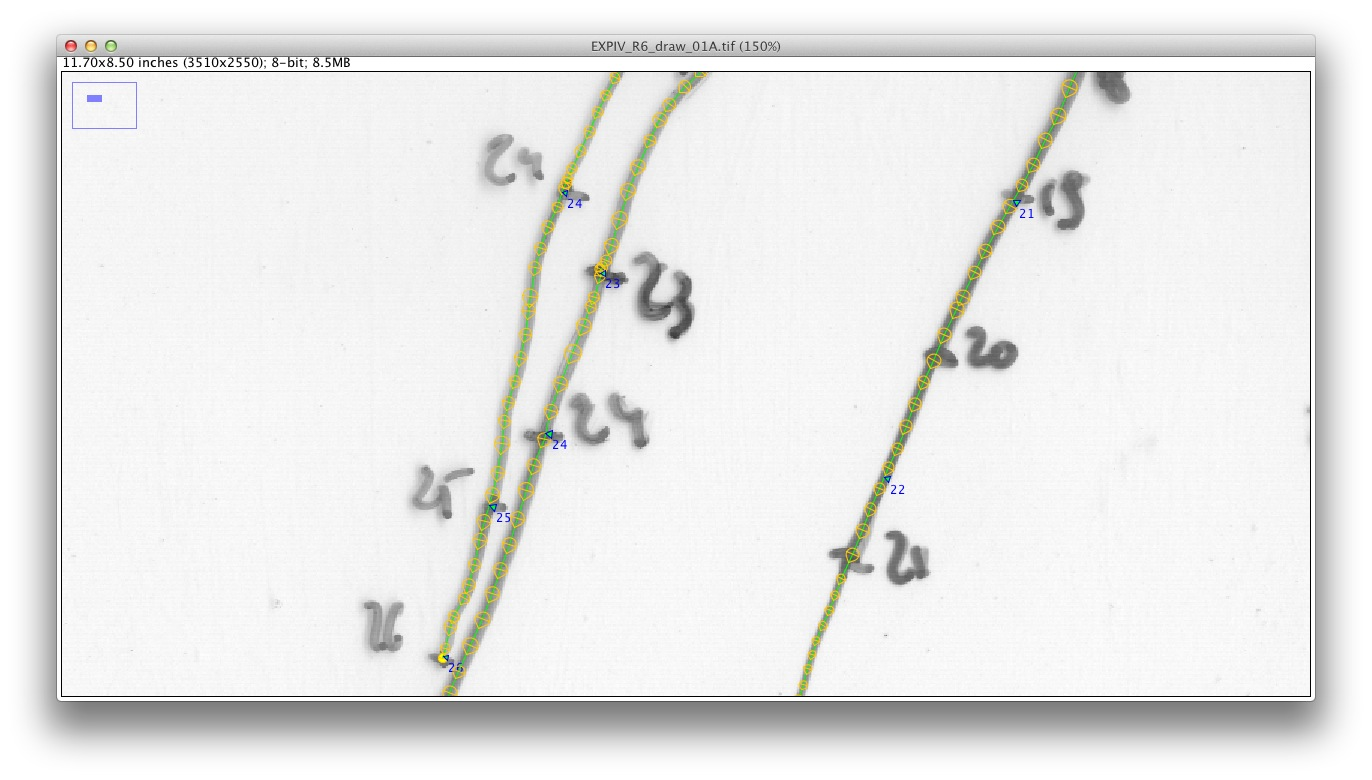
\includegraphics[width=10cm]{root_growth_drawing_close}
\caption[Root growth drawing and treatment]{\textbf{Example of hand drawing} of root growth with subsequent treatment in SmartRoot}
\label{root_growth_drawing_close}
\end{center}
\end{figure}


{\color{coolSection}\section{About the SmartRoot datafile}}

When closing a root image window, all graphic objects (name, nodes coordinates and diameter, marks) and the DPI setting are recorded in a separate file in XML format, referred to as the SmartRoot datafile. The datafile is named after the image name, with the .xml extension and is stored in the same directory as the image. When the image is opened later, the datafile is loaded and every root objects are automatically reloaded.\\

By default, the datafile is saved whenever an image is closing, unless you close explicitly the image with the command \verb|File>Quit without saving datafile| in the popup menu. If you modified the image content itself, for example by applying a smooth filter, ImageJ will ask you whether you want to save the image and or the datafile.\\

If you use the SaveAs command of ImageJ to save a copy of your image in a different folder and/or under a different name, a copy of the datafile is created as well and will be saved at the new location when the window is closed.\\
 
The \verb|File| item of the popup menu brings a submenu with a few actions related to the datafile:\\

\begin{description}
\item[Save DataFile:] Allows to directly save the datafile, without closing the image window (because SmartRoot is still a new software, it is recommended to regularly save the datafile this way)
\item[Clear DataFile:] Erase all root objects in memory.
\item[Use backup datafile:] Allows to use a previously saved datafile after a wrong manipulation of computer crash (see below).
\item[Quit without saving datafile] Name is self speaking.
\item[Import Seed Datafile] Allows to load the datafile of a different image (the "seed" image), provided the current image and the seed image have been registered with two anchor points (the process of registration is explained above). 
\end{description}

When a datafile is saved, the current datafile on disk is not replaced. Instead, its extension is changed to .xml01 (if an archive datafile .xml01 exists, it is renamed .xml02,… and so on until the .xml05 file which is deleted). To open an image with an archive datafile, right-click on the image name in the SmartRoot Explorer window and select the archive datafile you would like to use from the popup menu or use the right click on the image and choose \verb|File > Use backup datafile|.



\newpage
{\color{coolSection}\section{Using ImageJ functions and plugins in SmartRoot windows}}
\label{ijfunc}

It is in principle possible to use ImageJ functions and plugin on image windows that were opened with the SmartRoot user interface, with two exceptions:\\

\begin{enumerate}
\item Functions / plugins that change the \textbf{size} of the image will permanently inactivate the SmartRoot user interface in the modified image window. 
\item Functions / plugins that change the \textbf{type} of the image to anything else than 8-bit grayscale will prevent the the root detection algorithm to work properly (the rest of SmartRoot will be OK, though). The situation will get back to the normal as soon as the image type is reset to 8-bit grayscale.
\end{enumerate}

Image editing through ImageJ will not modify existing SmartRoot objects, simply because ImageJ does not know about root objects. It may therefore be necessary to re-trace these objects.\\

The process of saving images and datafiles becomes confusing when the user has edited an image that was opened in SmartRoot. Indeed, whenever an image has been edited, ImageJ brings up its own \verb|Save ? Yes-No-Cancel| dialog box when the image is closing. The user response only tells ImageJ whether the edited image should be saved, but does not tell SmartRoot whether the datafile should be saved. Whether the datafile is saved depends only on the way the image was closed. The only exception is the \verb|Save As| menu item of ImageJ, which stores both the image and datafile to a new location. In most instances, the user will not edit the image while working in SmartRoot and there should not be any problem.



{\color{coolSection}\section{Disclaimer}}

We put a lot of effort and time trying to make SmartRoot accurate, fast and user-friendly. However, we make no claims that SmartRoot is perfect and will work in every situation and with every image. You are advised to use it at your own risk. SmartRoot is still a work in progress and is still evolving. If you have any question, proposition, advise, please visit the our website (\url{www.uclouvain.be/smartroot}) to contact us.

%%%%%%%%%%%%%%%%%%%%%%%%%%%%%%%%%%%%%%%%%%%%%%%%%%%%%%%%%%%%%%%%
%%%%%%%%%%%%%%%%%%%%%%%%%%%%%%%%%%%%%%%%%%%%%%%%%%%%%%%%%%%%%%%%

\chapter{Troubleshooting}

There is FAQ section on SmartRoot's website (\url{www.uclouvain.be/en-smartroot}) covering the different troubles you might have using SmartRoot.

%{\color{coolSection}\section{While installing SmartRoot}}
%
%
%{\large \noindent \underline{\textbf{No database is found at the opening.}}}\\
%
%\noindent PROBLEM\\
%
%\noindent The \verb|Result| window display the following error message:
%
%\begin{Verbatim}[frame=single, commandchars=+\(\)]
%The ODBC datasource "SmartRoot" was not found.
%You will not be able to write to a database.
%\end{Verbatim}
%
%\noindent SOLUTION\\
%
%\noindent \textbf{Windows:} See section \ref{dbwin}\\
%\textbf{Mac OS X:} See section \ref{dbmac}\\
%\textbf{Linux:} See section \ref{dblin}
%
%
%
%\newpage
%{\color{coolSection}\section{While using SmartRoot}}
%
%{\large \noindent \underline{\textbf{Right click outside a root always leads to the menu of the same root.}}}\\
%
%\noindent  PROBLEM\\
%
%\noindent The root is not traced correctly and its borders are miscalculated leading to this interpretation errors. This happens when a node is inside an other one, typically, the last node inside the previous one.\\
%
%\noindent SOLUTION\\
%
%\noindent You can either find the problematic root (the one shown in the menu when you right click), find the wrong node and move/delete it, or directly delete the root (in the right click menu). \\
%
%\begin{figure}[htbp]
%\begin{center}
%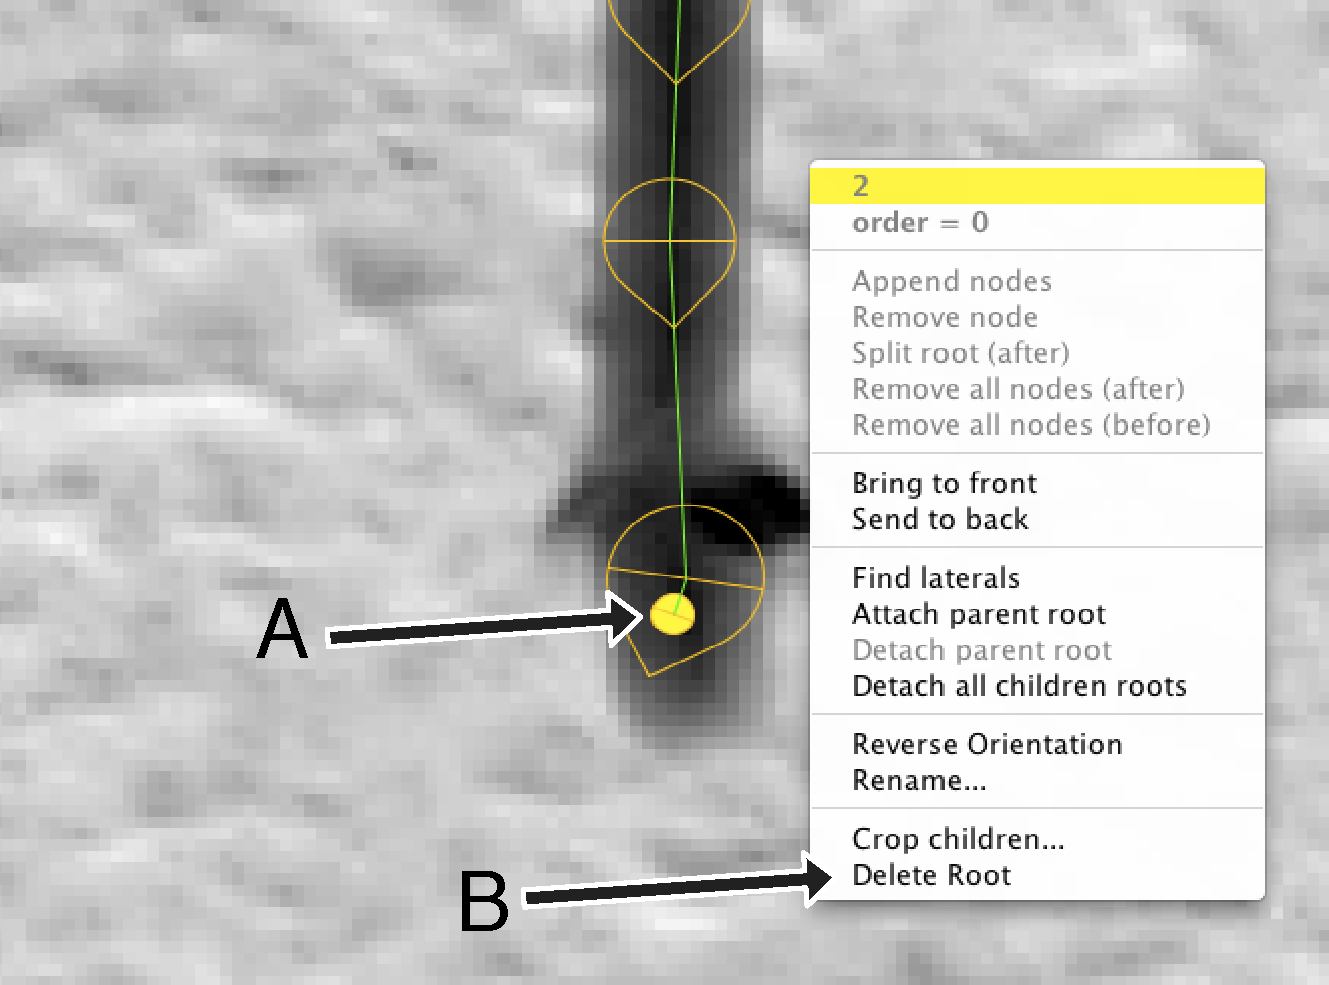
\includegraphics[width=8cm]{SR_bug_1}
%\caption[Miscalculation of root shape]{\textbf{Miscalculation of root shape}:  A. The last node of the root is inside the previous node, leading to a miscalculation of the root shape. B. To correct this bug, either delete the root or move the node outside the previous one.}
%\label{plot}
%\end{center}
%\end{figure}
%
%
%{\large \noindent \underline{\textbf{The Alt key is not working under Ubuntu.}}}\\
%
%\noindent  PROBLEM\\
%
%\noindent Ubuntu use the \verb|Alt| key to grab and move windows. SmartRoot use the same key to automatically trace roots.\\
%
%\noindent SOLUTION\\
%
%In order to use SmartRoot correctly, you have to change one Ubuntu parameter:\\
%
%\noindent Go to \verb|System > Preferences > Windows| and set the Movement key to Super.\\

%%%%%%%%%%%%%%%%%%%%%
%
%\chapter{Quick guide}
%
%{\color{coolSection}\section{Trace a root}}
%
%\begin{flushright}
%{\color{coolSection}\textsc{{\Large Manual tracing}}}
%\end{flushright}
%\noindent \fbox{\parbox{\linewidth}{ 
%\begin{enumerate}
%\item Select the {\color{red}Trace} tool
%\item Check {\color{red}Display nodes} and {\color{red}Display axis} in the Layer tab
%\item {\color{red}Click} inside a root to place a node. 
%\item Keep going until the end of the root
%\item {\color{red}Double click} to end the root
%\item Choose a name for the newly created root
%\end{enumerate}}}\\
%\begin{flushright}
%for more detailed information see section \ref{manualTrace}\\
%\end{flushright}
%\vspace{30pt}
%%
%\begin{flushright}
%{\color{coolSection}\textsc{{\Large Semi-automated tracing}}}
%\end{flushright}
%\noindent \fbox{\parbox{\linewidth}{ 
%\begin{enumerate}
%\item Select the {\color{red}Trace} tool
%\item Check {\color{red}Display nodes} and {\color{red}Display axis} in the Layer tab
%\item Maintain the {\color{red}Alt} key down
%\item {\color{red}Click} inside a root to trace it. 
%\item Choose a name for the newly created root
%\end{enumerate}}}\\
%\begin{flushright}
%for more detailed information see section \ref{autoTrace}\\
%\end{flushright}
%\vspace{30pt}
%%
%%
%\newpage
%{\color{coolSection}\section{Continue a root}}
%
%\begin{flushright}
%{\color{coolSection}\textsc{{\Large Manually continuing a root}}}
%\end{flushright}
%\noindent \fbox{\parbox{\linewidth}{ 
%\begin{enumerate}
%\item Select the {\color{red}Trace} tool
%\item Check {\color{red}Display nodes} and {\color{red}Display axis} in the Layer tab
%\item {\color{red}Right click} on the first or last node of an existing root and choose {\color{red}Append node}. 
%\item {\color{red}Click} inside the image to place a new node. 
%\item Keep going until the end of the root
%\item {\color{red}Double click} to end the root
%\end{enumerate}}}\\
%\begin{flushright}
%for more detailed information see section \ref{modify}\\
%\end{flushright}
%\vspace{30pt}
%%
%%
%%
%\begin{flushright}
%{\color{coolSection}\textsc{{\Large Automatically continuing a root}}}
%\end{flushright}
%\noindent \fbox{\parbox{\linewidth}{ 
%\begin{enumerate}
%\item Select the {\color{red}Trace} tool
%\item Check {\color{red}Display nodes} and {\color{red}Display axis} in the Layer tab
%\item Hold the {\color{red}Alt} key down
%\item {\color{red}Click} on an existing node and {\color{red}drag} it a bit further. 
%\end{enumerate}}}\\
%\begin{flushright}
%for more detailed information see section \ref{modify}\\
%\end{flushright}
%\vspace{30pt}
%%
%%
%%
%\newpage
%{\color{coolSection}\section{Modify roots}}
%
%\begin{flushright}
%{\color{coolSection}\textsc{{\Large Modifying nodes}}}
%\end{flushright}
%\noindent \fbox{\parbox{\linewidth}{ 
%\vspace{10pt}
%{\color{red}Right click} on an existing node. Choose on of the following action:
%\begin{description}
%\item[Append nodes:] Continue tracing in manual mode 
%\item[Split root:] Split a root in two new roots.
%\item[Remove node:] Remove the selected node.
%\item[Remove all nodes (after):] Discard all node located distal to the selected node.
%\item[Remove all nodes (before):] Discard all node located proximal to the selected node.\\
%\end{description}}}\\
%\begin{flushright}
%for more detailed information see section \ref{modify}\\
%\end{flushright}
%\vspace{30pt}
%%
%%
%\begin{flushright}
%{\color{coolSection}\textsc{{\Large Modifying roots}}}
%\end{flushright}
%\noindent \fbox{\parbox{\linewidth}{ 
%\vspace{10pt}
%{\color{red}Right click} inside an existing root. Choose on of the following action:
%\begin{description}
%\item[Bring to front:] Bring the selected root to the front of the list of roots. 
%\item[Send to back:] Send the selected root to the back of the list of roots.
%\item[Find laterals:] Check along the root axis for lateral roots creation. 
%\item[Attach parent root:] Set a parent for the current root.
%\item[Detach parent root:] Remove the relationship between a root and its parent.
%\item[Detach children roots:] Remove the relationship between a root and all its children.
%\item[Rename root:] Change the name of the selected root.
%\item[Delete a root:] Remove the whole root.
%\item[Reverse orientation:] Reverse the root orientation.
%\item[Crop children:] Cut all roots whose first node is within the area of the selected root.
%\end{description}}}\\
%\begin{flushright}
%for more detailed information see section \ref{modify}\\
%\end{flushright}
%\vspace{30pt}
%
%\newpage
%\begin{flushright}
%{\color{coolSection}\textsc{{\Large Connecting two existing roots}}}
%\end{flushright}
%\noindent \fbox{\parbox{\linewidth}{ 
%\begin{enumerate}
%\item Select the {\color{red}Trace} tool
%\item Check {\color{red}Display nodes} and {\color{red}Display axis} in the Layer tab
%\item {\color{red}Right click} on the first or last node of an existing root and choose {\color{red}Append node}. 
%\item {\color{red}Right click} on the first or last node of an other existing root. 
%\end{enumerate}}}
%\begin{flushright}
%for more detailed information see section \ref{connecting}\\
%\end{flushright}
%\vspace{30pt}
%
%\begin{flushright}
%{\color{coolSection}\textsc{{\Large Escaping the centering mechanism}}}
%\end{flushright}
%\noindent \fbox{\parbox{\linewidth}{ 
%\begin{enumerate}
%\item Select the {\color{red}Trace} tool
%\item Check {\color{red}Display nodes} and {\color{red}Display axis} in the Layer tab
%\item Hold the {\color{red}Control} key down and move a node for a {\color{coolSection}Diameter freeze}
%\item Hold the {\color{red}Shift} key down and move a node for a {\color{coolSection}Align to border}
%\item Combine {\color{red}Control}, {\color{red}Shift} and {\color{red}Alt} keys.
%\end{enumerate}}}
%\begin{flushright}
%for more detailed information see section \ref{connecting}\\
%\end{flushright}
%
%
%
%\newpage
%{\color{coolSection}\section{Root window's tabs}}
%\begin{flushright}
%{\color{coolSection}\textsc{{\Large Layers tab}}}
%\end{flushright}
%\noindent \fbox{\parbox{\linewidth}{ 
%\begin{center}
%\begin{tabular}{lp{0.6\linewidth}}
%\multirow{2}{*} {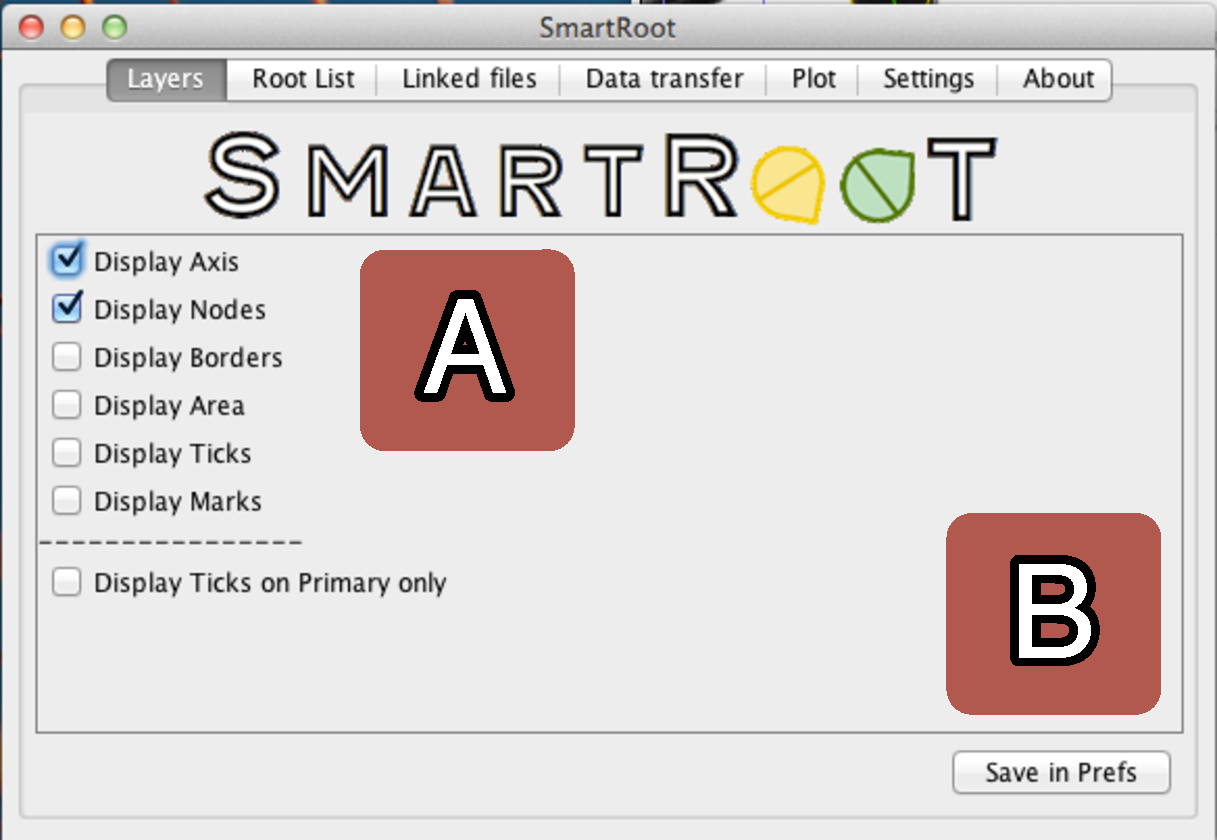
\includegraphics[width=0.3\linewidth]{layers}} & \textbf{A.} Type of layers.\\ 
% & \textbf{B.} Save your preferences.\\  \vspace{45pt}
%\end{tabular}
%\end{center}}}
%\begin{flushright}
%for more detailed information see section \ref{chapdisp}\\
%\end{flushright}
%\vspace{20pt}
%
%
%\begin{flushright}
%{\color{coolSection}\textsc{{\Large Root list tab}}}
%\end{flushright}
%\noindent \fbox{\parbox{\linewidth}{ 
%\begin{center}
%\begin{tabular}{lp{0.5\linewidth}}
%\multirow{7}{*} {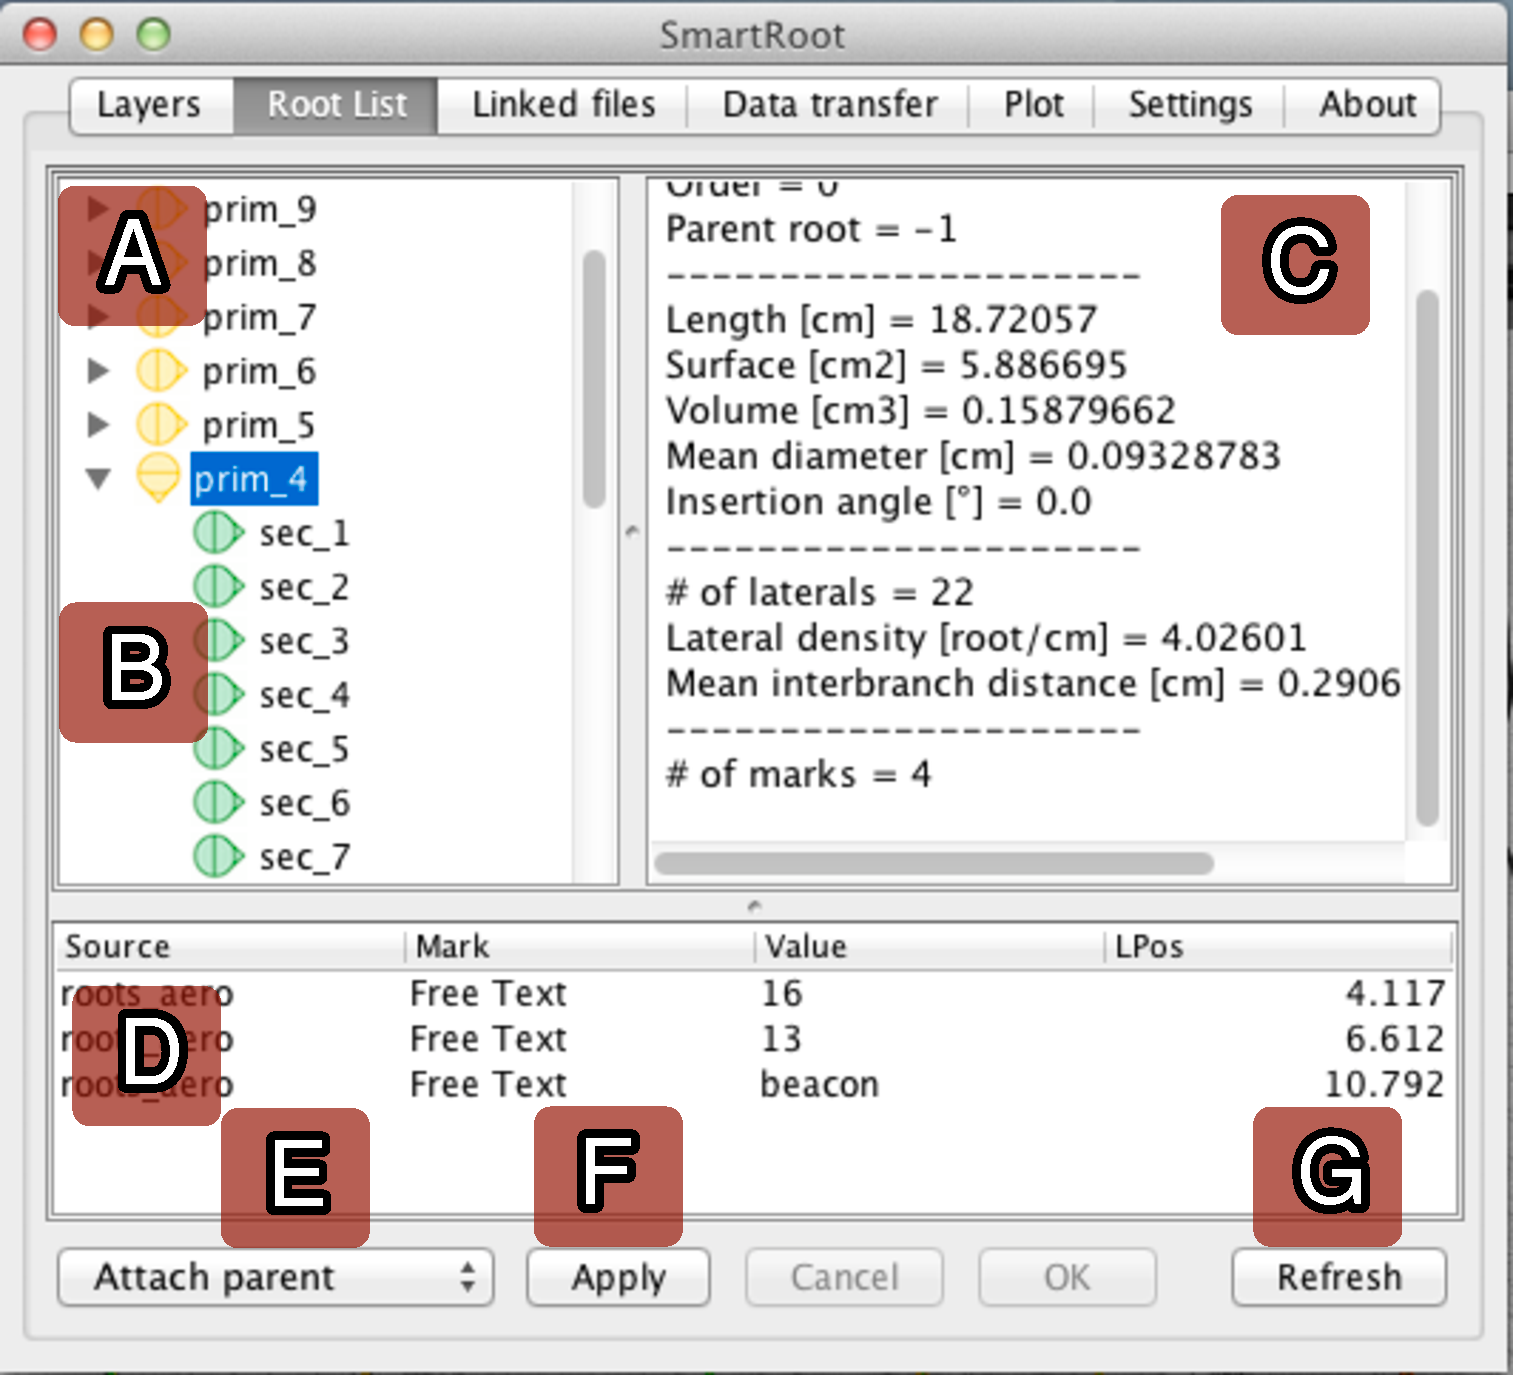
\includegraphics[width=0.4\linewidth]{root_list}} & \textbf{A.} Primary roots, in yellow.\\ 
% & \textbf{B.} Secondary roots, in green.\\ 
% & \textbf{C.} Informations about the selected root(s). \\ 
% & \textbf{D.} Marks of the selected root.\\ 
% & \textbf{E.} Perform actions on the selected root(s).\\
% & \textbf{F.} Validate the chosen action.\\ 
% &\textbf{G.} Refresh the root list \\
%\end{tabular}
%\end{center}
%\begin{center}
%\vspace{65pt}\rule{0.8\linewidth}{1pt}\vspace{15pt}
%\begin{tabular}{p{0.1\linewidth}p{0.8\linewidth}}
%\textbf{Actions:} & Delete root(s) | Delete mark(s) | Rename root\\
%& Attach parent | Detach parent | Detach child(ren) | Find laterals
%\end{tabular}
%\end{center}}}
%\begin{flushright}
%for more detailed information see section \ref{rootlist}\\
%\end{flushright}
%\vspace{20pt}
%
%\begin{flushright}
%{\color{coolSection}\textsc{{\Large Linked files tab}}}
%\end{flushright}
%\noindent \fbox{\parbox{\linewidth}{ 
%\begin{center}
%\begin{tabular}{lp{0.5\linewidth}}
%\multirow{2}{*} {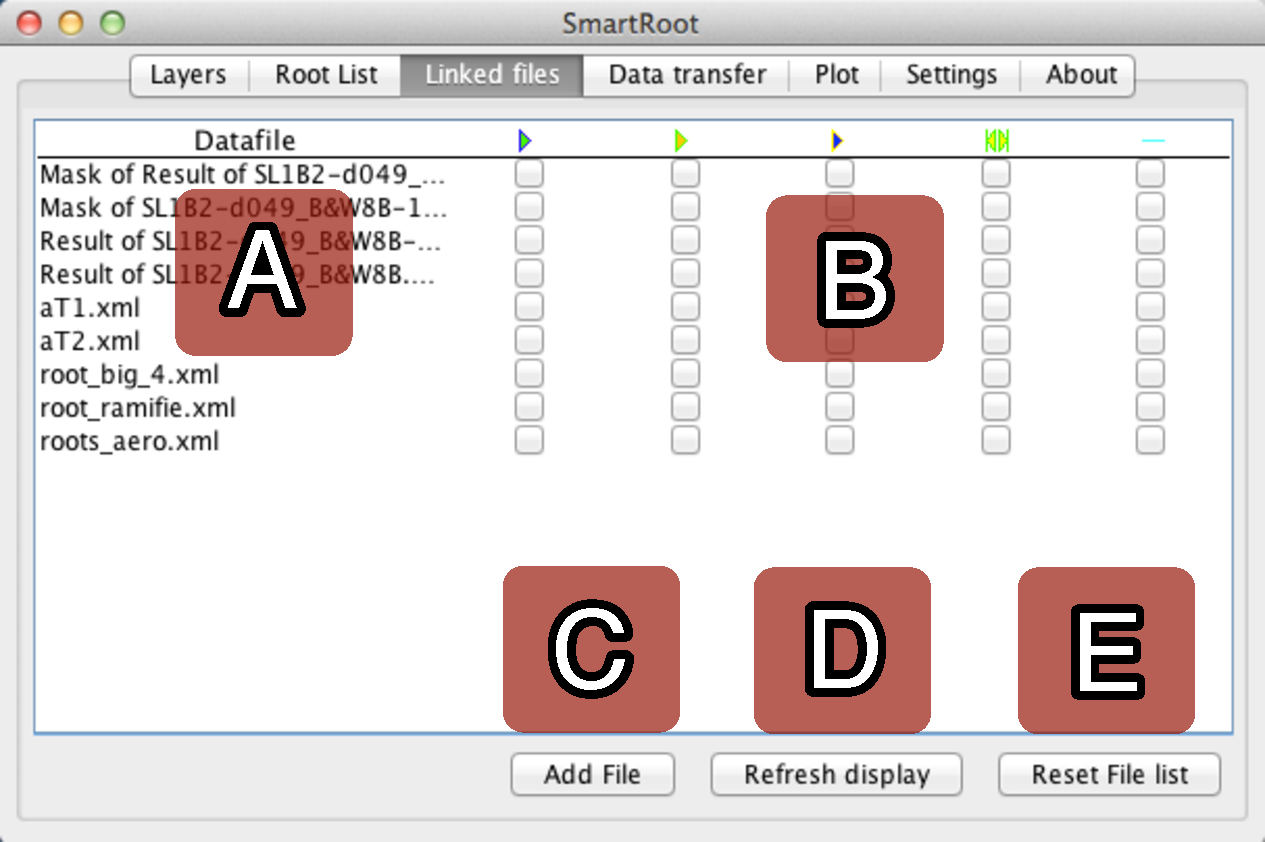
\includegraphics[width=0.4\linewidth]{linked_files}} & \textbf{A.} Files to link.\\ 
% & \textbf{B.} Marks to link.\\  
% & \textbf{C.} Add a file to the list.\\
% & \textbf{D.} Refresh the image display.\\
% & \textbf{E.} Refresh the list display.\\      \vspace{40pt}
%\end{tabular}
%\end{center}}}
%\begin{flushright}
%for more detailed information see section \ref{chaplink}\\
%\end{flushright}
%\vspace{20pt}
%
%
%
%\begin{flushright}
%{\color{coolSection}\textsc{{\Large Data transfers tab}}}
%\end{flushright}
%\noindent \fbox{\parbox{\linewidth}{ 
%\begin{center}
%\begin{tabular}{lp{0.5\linewidth}}
%\multirow{4}{*} {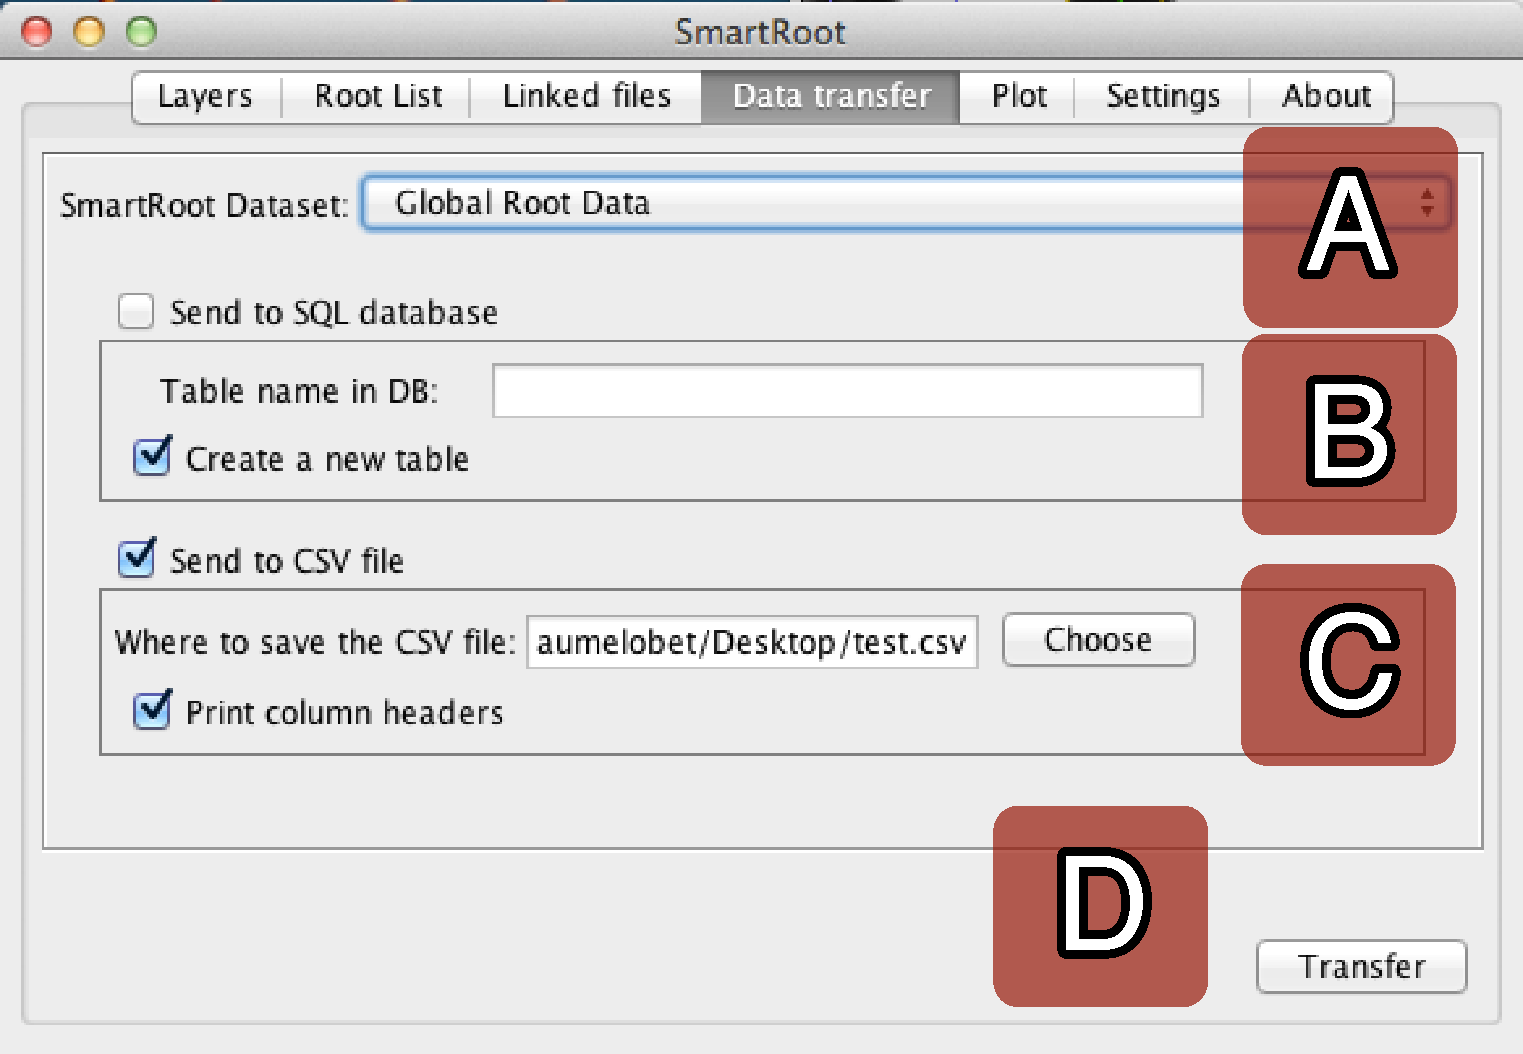
\includegraphics[width=0.4\linewidth]{data_transfers}} & \textbf{A.} List of SmartRoot datasets.\\ 
% & \textbf{B.} Export to SQL. \\ 
% & \textbf{C.} Export to CSV\\ 
% & \textbf{D.} Transfers button.\\ \vspace{40pt} 
%\end{tabular}
%\end{center}
%\begin{center}
%\vspace{20pt}\rule{0.8\linewidth}{1pt}\vspace{15pt}
%\begin{tabular}{p{0.1\linewidth}p{0.8\linewidth}}
%\textbf{Datasets:} & Global Root Data | All marks | Root Nodes | Root Length density\\
%\end{tabular}
%\end{center}}}
%\begin{flushright}
%for more detailed information see section \ref{chaptrans}\\
%\end{flushright}
%\vspace{20pt}
%
%\begin{flushright}
%{\color{coolSection}\textsc{{\Large Plot tab}}}
%\end{flushright}
%\noindent \fbox{\parbox{\linewidth}{ 
%\begin{center}
%\begin{tabular}{lp{0.6\linewidth}}
%\multirow{5}{*} {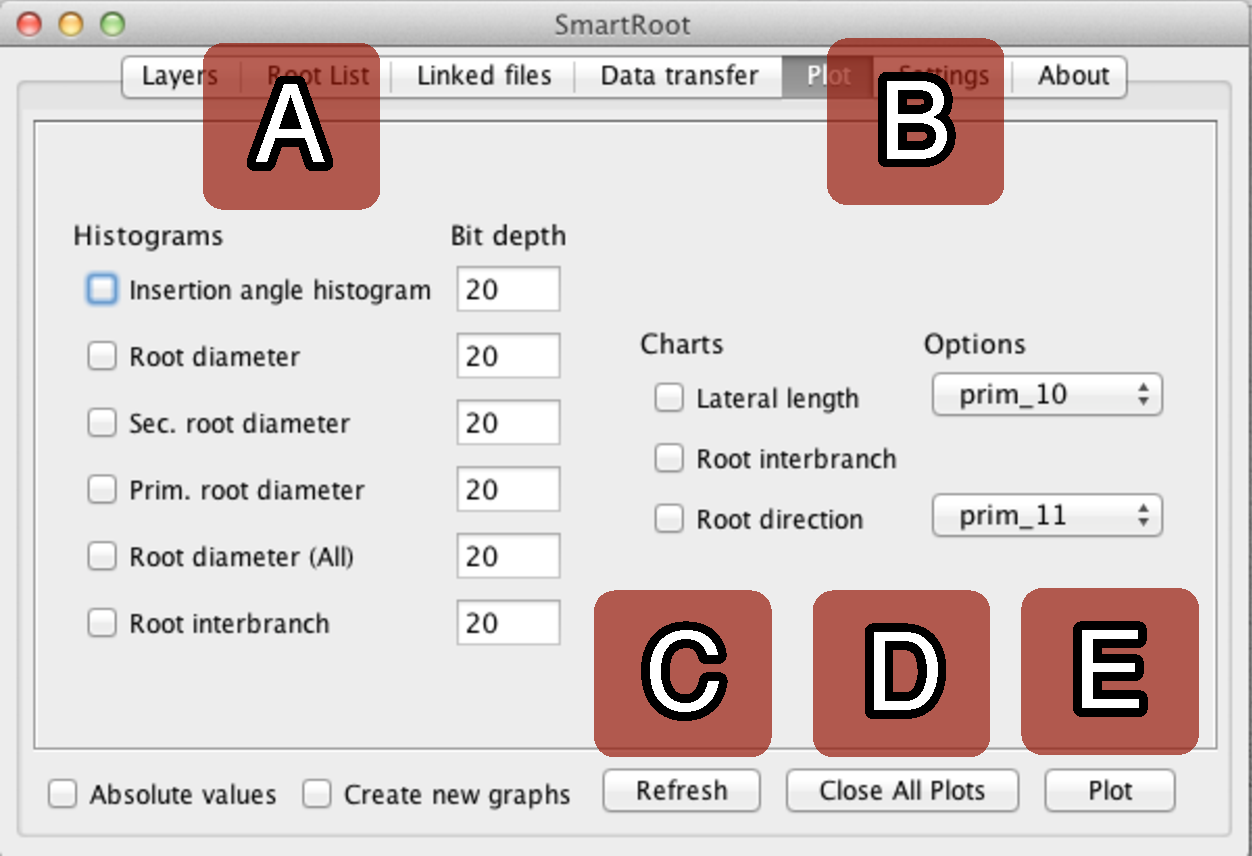
\includegraphics[width=0.4\linewidth]{SR_plot}} & \textbf{A.} Histograms (see section \ref{hist}).\\ 
% & \textbf{B.} Charts (see section \ref{chart}).\\ 
% & \textbf{C.} Refresh button. \\ 
% & \textbf{D.} Close all plots.\\ 
% & \textbf{E.} Plot the selected charts and histograms.\\ \vspace{35pt}
%\end{tabular}
%\end{center}}}
%\begin{flushright}
%for more detailed information see section \ref{chapplot}\\
%\end{flushright}
%\vspace{20pt}
%
%
%\begin{flushright}
%{\color{coolSection}\textsc{{\Large Settings tab}}}
%\end{flushright}
%\noindent \fbox{\parbox{\linewidth}{ 
%\begin{center}
%\begin{tabular}{lp{0.6\linewidth}}
%\multirow{5}{*} {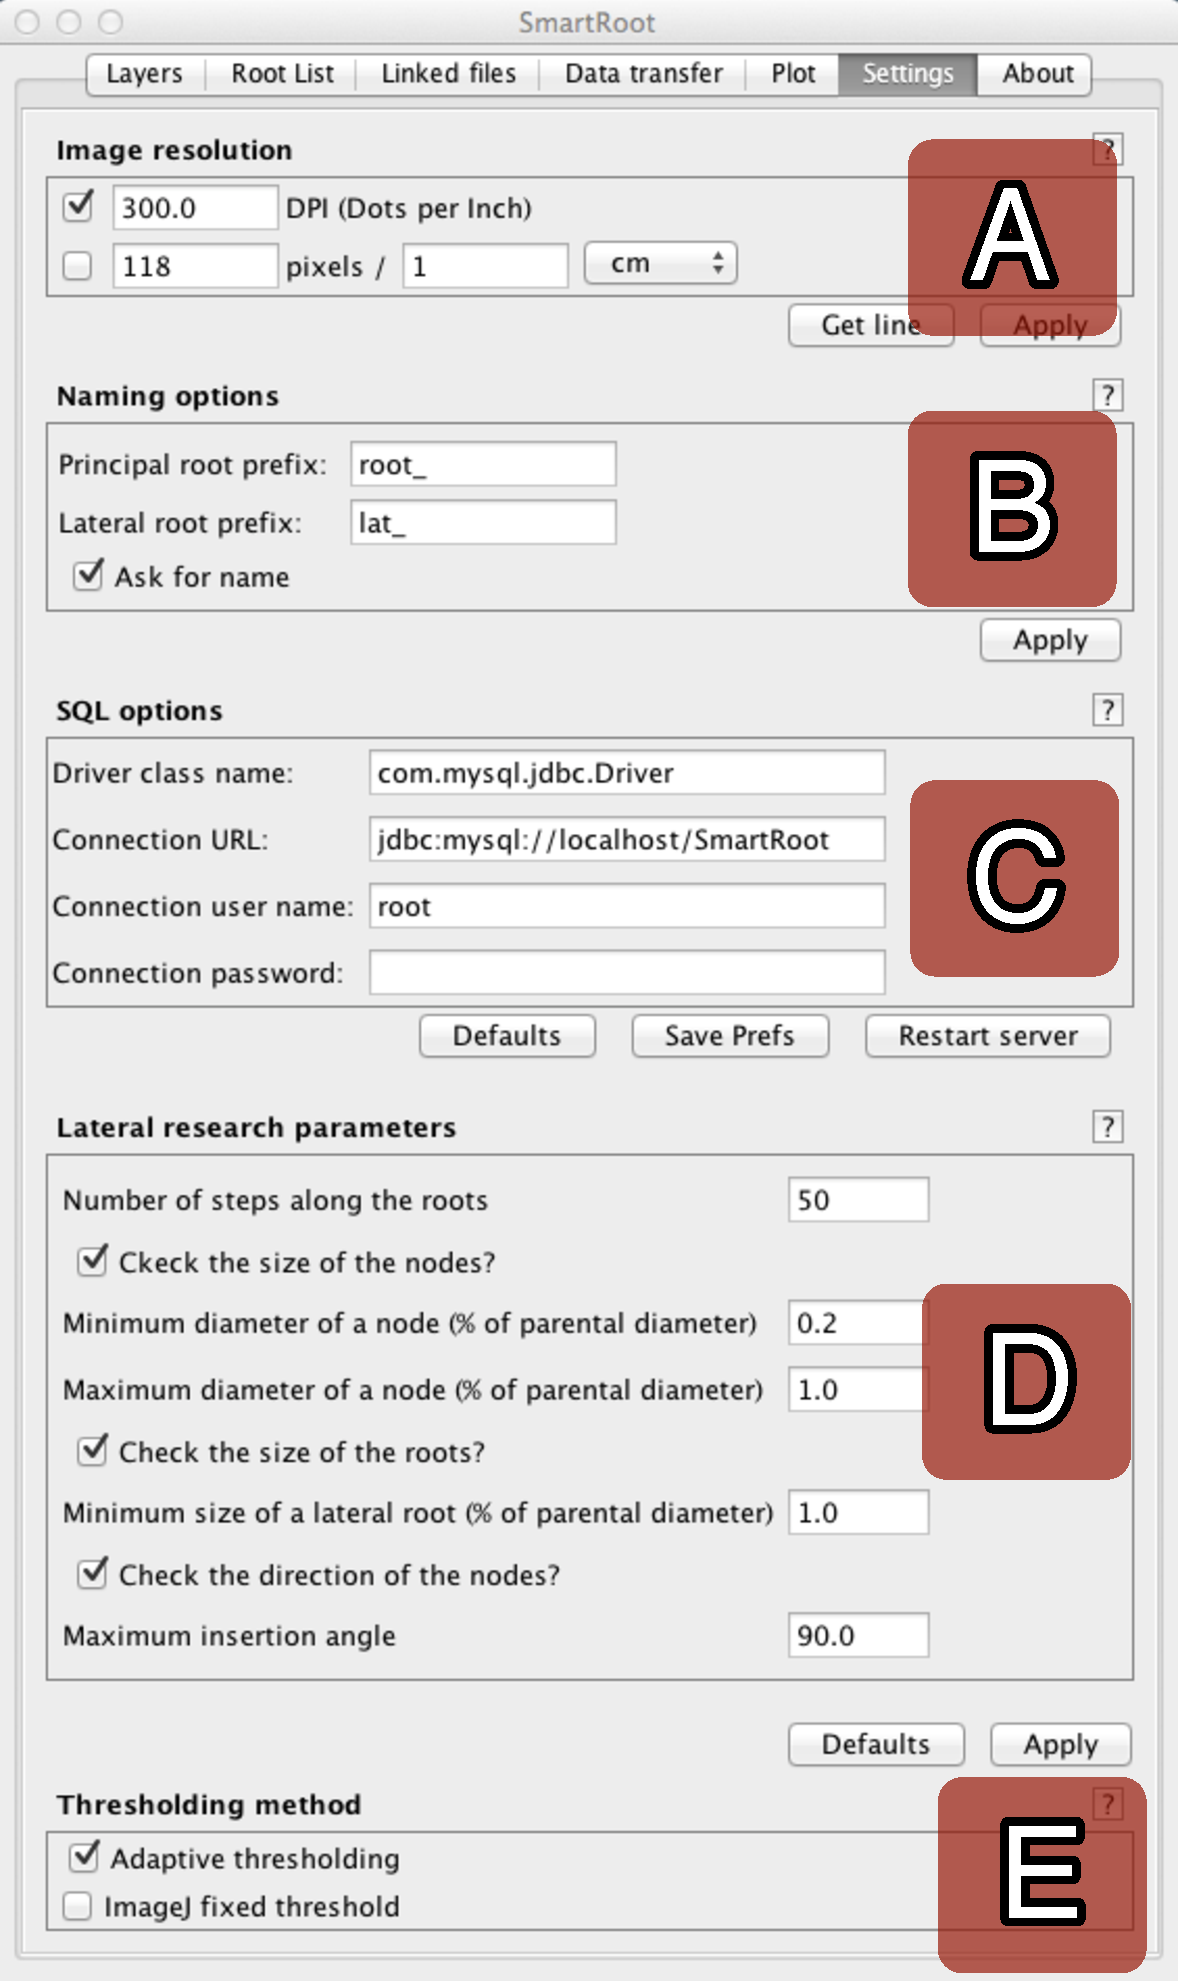
\includegraphics[width=0.2\linewidth]{settings}} & \textbf{A.} Image resolution (section \ref{resolution_options}).\\ 
% & \textbf{B.} Naming options (section \ref{name_options}).\\ 
% & \textbf{C.} SQL options (section \ref{sql_options}). \\ 
%& \textbf{D.} Lateral finding options (section \ref{lat_options}). \\ 
% & \textbf{E.} Thresholding options (section \ref{th_options}). \\ \vspace{70pt}
%\end{tabular}
%\end{center}}}
%\begin{flushright}
%for more detailed information see section \ref{chapsettings}\\
%\end{flushright}



\printindex


\end{document}








